\documentclass[11pt, a4paper]{memoir}
\usepackage[utf8]{inputenc}
\usepackage[english, science, dropcaps, hyperref, submissionstatement]{ku-frontpage}

% Math-related packages
\usepackage{amsmath, amssymb, amsfonts, mathrsfs, latexsym, mathtools}
\usepackage{ntheorem}
\usepackage{tikz}
\usepackage[framemethod=TikZ]{mdframed}
\usepackage{centernot}
\usepackage{tikz-cd}

% Miscellaneous packages
\usepackage{enumitem}
\usepackage{float}
\usepackage{xcolor}
\usepackage{etoolbox}
\usepackage[most]{tcolorbox}
\tcbuselibrary{theorems, skins, breakable}
\usepackage{ulem}
\usepackage{microtype}
\usepackage{setspace}
\usepackage{graphicx, caption}
\usepackage{chngcntr}
\usepackage{cleveref}
\definecolor{emphcolor}{HTML}{901A1E} % Using kuRed

\newcommand{\coloremph}[1]{\textcolor{emphcolor}{\emph{#1}}}

\DeclareCaptionStyle{mystyle}{%
  font=it, % Italif font
  labelsep=space, % Use space instead of colon
  justification=RaggedRight % Left-align the caption
}
\captionsetup{style=mystyle}
\captionsetup{belowskip=-15pt}

\crefformat{footnote}{#2\footnotemark[#1]#3}
\counterwithout{figure}{chapter}

% Theorem-like environments with italicized text
\theoremstyle{break}
\theoremheaderfont{\normalfont\bfseries}
\theorembodyfont{\itshape} % Italicized text
\theoremseparator{.}

\newtheorem{thm}{Theorem}
\newtheorem{prop}{Proposition}
\newtheorem{cor}{Corollary}
\newtheorem{lem}{Lemma}

% Definition environment with non-italicized text
% Definition environment with non-italicized text
\theoremstyle{break}
\theoremheaderfont{\normalfont\bfseries\vspace{3pt}}
\theorembodyfont{\normalfont} % Non-italicized text
\theoremseparator{.}
\newtheorem{innerdefn}{Definition}

\newenvironment{defn}
  {\begin{innerdefn}}
  {\ensuremath{\circ}\end{innerdefn}}
  

\newtheorem{inneralg}{Algorithm}
\newenvironment{alg}{\begin{inneralg}}{\ensuremath{\circ}\end{inneralg}}  

% Alternative definition environment
\definecolor{kuRed}{HTML}{901A1E}
\definecolor{kuGray}{HTML}{666666}
\definecolor{lightKuGray}{HTML}{FFE8D1}

% Define the 'mydefinition' tcolorbox environment
\newtcolorbox[auto counter,number within=chapter]{mydefinition}[2][]{
  breakable, % Allows the box to break across pages
  colback=lightKuGray!80, % Background color for the entire box
  colframe=lightKuGray!80, % Frame color
  coltitle=black, % Text color for the title
  title={\textbf{Definition~\thetcbcounter\ (#2)\ #1}}, % Title with bold "Definition" and optional description
  fonttitle=\bfseries, % Make the title text bold
  enhanced,
  sharp corners,
  boxrule=1pt, % Width of the frame lines
  top=8pt, % Top space within the box (inside the frame)
  bottom=8pt, % Bottom space within the box (inside the frame)
  left=8pt, % Left space within the box (inside the frame)
  right=8pt, % Right space within the box (inside the frame)
  toprule=10pt,
  before=\vskip15pt,
  after=\vskip15pt,
  #1 % For specifying additional options
}

\theoremstyle{nonumberplain}
\theoremsymbol{\ensuremath{\square}} 
\newtheorem{proof}{Proof}

% Custom commands and math operators
\newcommand{\mN}{\mathbb{N}}
\newcommand{\mZ}{\mathbb{Z}}
\newcommand{\mQ}{\mathbb{Q}}
\newcommand{\mR}{\mathbb{R}}
\newcommand{\mD}{\mathbb{D}}
\newcommand{\mH}{\mathbb{H}}
\newcommand{\mC}{\mathbb{C}}
\newcommand{\mP}{\mathbb{P}}
\newcommand{\mF}{\mathbb{F}}
\newcommand{\abs}[1]{\left| #1\right|}
\newcommand{\norm}[1]{\left\lVert#1\right\rVert}
\newcommand{\indep}{\perp \!\!\! \perp}

\DeclareMathOperator{\pa}{pa}
\DeclareMathOperator{\de}{de}
\DeclareMathOperator{\nei}{ne}
\DeclareMathOperator{\bd}{bd}
\DeclareMathOperator{\nd}{nd}
\DeclareMathOperator{\an}{An}
\DeclareMathOperator{\rank}{rank}
\DeclareRobustCommand{\firstsecond}[2]{#2}

% Other settings
\setlength\arraycolsep{2 pt}
\setcounter{tocdepth}{2}
\setcounter{secnumdepth}{1}
\setlength{\jot}{8pt}

\assignment{Master's thesis}

% The following are only needed if the \author, \title, \subtitle, and \date
% commands are not patchable. See the readme for more information.
% \frontpageauthor{Alex Author}
% \frontpagetitle{A concise but nevertheless\\precise and interesting title}
% \frontpagesubtitle{An intruiging subtitle}
% \frontpagedate{Submitted: \today}

\frontpagetitle{Causal Inference in Dynamic Systems}
\subtitle{Convergent Cross Mapping and Alternative Approaches}
\frontpageauthor{Rasmus Juhl Christensen}
\frontpagedate{Submitted: \today}
\advisor{Advisor: Niels Richard Hansen}
\frontpageimage{example.png}

\kupdfsetup{A concise but nevertheless precise and interesting title - An intruiging subtitle}{}{Alex Author}

\begin{document}
\begingroup
  \fontencoding{T1}\fontfamily{LinuxLibertineT-OsF}\selectfont
  \maketitle
\endgroup

\section*{Abstract}

\subsubsection*{Description from contract}
The main goal of the project is to investigate dynamic systems for time series and the effectiveness of convergent cross mapping (CCM) to detect causality in this framework compared to other approaches on the basis of a reference model. Drawing on the paper "Detecting Causality in Complex Ecosystems" (2012) and "Distinguishing time-delayed causal interactions using convergent cross mapping", the project will explore the theoretical foundations, practical applications and potential shortfalls of CCM and its link to more classical methods in causality.\\\\
Reference 1: Detecting Causality in Complex Ecosystems. George Sugihara, Robert May, Hao Ye, Chih-hao Hsieh, Ethan Deyle, Michael Fogarty and Stephan Munch. Science , 26 October 2012, New Series, Vol. 338, No. 6106 (26 October 2012), pp. 496-500.
Reference 2: Distinguishing time-delayed causal interactions using convergent cross mapping. Hao Ye, Ethan R. Deyle, Luis J. Gilarranz \& George Sugihara. Scientific Reports volume 5, Article number 14750, 2015.\\\\
 
\textit{Front page image generated by Chaoscope.}
\newpage
\tableofcontents


\vfill
\noindent All code and data used in this project is available at \url{github.com/juhlc/speciale}.

\normalem

\newpage

\section*{Introduction}
Causality is a cornerstone of understanding in various scientific domains, setting the stage for profound realizations. At its core, causal inference addresses the intricate dance between correlation and causation. While correlation hints at a mutual relationship between two variables, causation pushes us into the territory of assertion — \textit{does one variable truly influence the other?} Traditional statistics employs randomization as a useful tool. Imagine a medical scenario where you can control who receives a treatment: If you can ensure that it is perfectly random who receives the treatment and patients receiving the treatment consistently show improvement compared to those who don't, we can attribute that difference to the treatment. However, when variables are merely observed without that level of control, establishing causation becomes more complex. Causal statistics thus requires another level of statistical modelling, because we want to reason about what happens when intervening in the process.\\\\
This thesis delves into the vibrant world of causal relationships in dynamic systems. Granger causality, a seminal and widely used concept in causal analysis of time series, yields one approach to causal inference in time-dependent data. It is based on the thoughts of \cite{Granger}, and it posits that if the past of a variable $C$ contains unique information about another variable $E$, the variable $C$ is said to 'Granger-cause' the other variable $E$. This approach to causal inference is based on prediction and at its core, it operates on the principle that cause precedes effect, and therefore, knowledge of the cause can enhance the predictability of the effect. However, while Granger causality offers a framework for assessing causality in probabilistic settings, it encounters challenges in deterministic systems. Dynamic systems, by their nature, have variables that are interconnected and governed by underlying structures. This interconnectedness means that information about one variable can often be extracted from another due to the system's inherent dynamics, rather than any direct causal link.\\\\
A case in point is the result from Takens (1981), which suggests that observing a single variable from a dynamic system might be sufficient to capture the entire system's dynamics. This interconnectedness can lead Granger causality to mistakenly identify causal links where none exist. Enter now the deterministic systems' viewpoint: Instead of relying on simple prediction improvement as a marker of causality, we focus on the inherent information within variables. If variable 
$C$ causes variable $E$, then $E$ should encapsulate information about the dynamics of $C$. However, $C$ would not necessarily contain comprehensive information about $E$ because the dynamics of $E$ not imposed by $C$ would not be reflected in the values of $C$. This perspective flips Granger causality on its head: while Granger causality might predict the effect 
$C$ using the cause $E$, a deterministic viewpoint effectively suggests the opposite. \\\\
This distinction, subtle yet profound, reshapes our understanding of causality in dynamic systems. As we proceed, we will delve deeper into the theoretical underpinnings of this perspective, unpacking its implications and potential applications. In particular, this is the insight that leads to the Convergent Cross Mapping approach introduced by \cite{Sugihara}, which in some sense will be the point of departure of this thesis and will be the primary among the methods based on Takens' theorem. This approach is detailed in Chapter \ref{chapTaken}.\\\\
Yet, while the deterministic paradigm offers a fascinating lens to understand causality, there is an inherent limitation. Real-world systems, especially in fields like economics, biology, and climate science, are rife with unpredictable fluctuations. These fluctuations cannot always be attributed solely to the endogenous dynamics of the system. No matter how meticulously one captures the deterministic dynamics, there will always be elements of seeming randomness and external influences that a purely deterministic model would struggle to account for. We return thus to stochastic processes. By reintroducing a stochastic element into our models, we can more faithfully represent the unpredictability and variability inherent in real-world systems. Stochasticity provides a framework to account for the 'noise' that isn't explained by the deterministic components of a system. Moreover, it's a nod to the humility of our modeling efforts – recognizing that there are always aspects of complex systems that are beyond our current understanding or are inherently random. 
In the subsequent chapters, we will delve deeper into the fusion of deterministic dynamics with stochastic processes using  a mixture of simulation based methods and theoretical considerations seeking a harmonious balance that brings us closer to understanding the multifaceted nature of causality in dynamic systems.

\section*{Introduction}
In this chapter, we introduce an approach to causal inference in dynamic systems, drawing inspiration from \cite{Sugihara}. In this thesis, we will adopt a rather broad definition of dynamical systems. We will envision them as objects tracing the evolution of a set of variables of interest over time under the assumption of some deterministic and suitably regular non-linear relationship. A more detailed and precise definition will be presented in subsequent sections.\\\\ The \textit{Convergent Cross Mapping (CCM)} method of \cite{Sugihara} anchors this chapter, but we will give a broader introduction to state space reconstruction based methods given a shared theoretical foundation. The theory of state space reconstruction is formulated in the language of differential topology, and Takens' theorem of 1981, \cite{Takens}, is a cornerstone. Takens' theorem solves the problem of constructing embeddings of high-dimensional systems from a single variable under a set of fairly general assumptions. In our context, such an embedding is a \textit{state space reconstruction} of a dynamic system. We will explore this concept further within this chapter.\\\\
To illustrate the challenge of causal inference in complex dynamic systems, we will use the example of \cite{Sugihara} regarding the interactions between anchovies, sardines and sea surface temperature in the California Current ecosystem. This real-world example serves as a backdrop for the more theoretical nature of the rest of this chapter. We will also introduce the causal framework of structural causal models inspired by the account of \cite{Peters}. This framework not only offers a model for causal inference but also a guideline for formulating a causal language for models in a deterministic setting. Due to the inherent differences between the mathematical theory used to formulate models in stochastic and deterministic settings, we will aim to relate the underlying assumptions in each setting. However, we will inevitably encounter some conceptual problems, as any attempt to translate the philosophical concept of causality into mathematical terms will be endowed with non-trivial complications and notable exceptions. We will discuss these problems throughout as they arise and try to be explicit about the assumptions and potential problems of the causal framework chosen in this thesis. We will also briefly discuss alternative formulations less conducive to overly strong interpretations.\\\\
We will then turn to a more stringent introduction to the theory of embeddings. This will allow us to formulate the main theoretical results of this thesis in full detail laying bare the explicit assumptions and results concerning identifiability of causal links in our framework. We will emphasize the definitions and proof techniques used to formulate and prove Takens' theorem and discuss some expansions and alternative formulations. Using the work of \cite{mathFound}, this paves the way for the main theorem of this thesis, namely a complete characterization of the causal inference possible from state space reconstruction in dynamic systems. This will complete the introduction of the theoretical set-up of the central model of this thesis.\\\\
Concluding this chapter, we present a thorough account of CCM and its alternatives and extensions. Notably, we discuss the methods suggested by \cite{Ye2015} and \cite{Leng2020}, which address problems not resolved by CCM, respectively that of distinguishing bidirectional causality and unidirectional causality in systems with some degree of synchronicity; and that of identifying the causal chain in a system knowing the causal directions between causally related variables. We will also cover some related methods that are more rooted in machine learning but still use state space reconstruction for causal inference, albeit with less explicit theoretical foundation. We will then revisit the California Current example from the beginning and analyse it using the developed theory. However, it is crucial to remember that that the theory of this chapter applies only to purely deterministic systems, and real-world examples often have a mix of deterministic and stochastic structures. We will address this limitation in subsequent chapters, by considering a set-up replacing systems of differential equations with systems of stochastic differential equations, and analysing the effect of measurement noise or stochastic influences on the effectiveness of our methodology.
\newpage

\section*{An Example}
In this section, we will briefly discuss a real-world example concerning sardine and anchovy populations in the California Current System. This is the same example considered by \cite{Sugihara} and so we aim to use the same data for our analysis with the modification that we include data from the period 2012-2022 as well. We will use the following data:
\begin{itemize}
\item Pacific sardine (\textit{Sardinops sagax}) California fish market catch landings recorded monthly in pounds in the period January 1928 up to and including December 2022. There are 12 months with redacted data.\footnote{\label{note1}Data from January 1928 up to and including December 2002 is obtained from from \textit{ERDDAP} at \cite{oldData}, and data from January 2003 up to and including December 2022 is obtained directly from \cite{newData}.}
\item Northern anchovy (\textit{Engraulis mordax}) California fish market catch landings recorded monthly in pounds in the period January 1928 up to and including December 2022. There are 34 months with redacted data.\cref{note1} 
\item  Sea-surface temperature (SST) measured daily in $\text{C}^\circ$ as an average between temperatures measured at the two sites Scripps Pier Shore Station and Balboa Pier Shore Station in the period August 22, 1916 up to and including December 31, 2022. There are 458 days without any measurements at either site.\footnote{The data from Scripps Pier is maintained by \cite{Scripps} and covers the period from August 22, 1916 up to and including December 31, 2022. The data from Newport Pier is maintained by \cite{Newport} and covers the period November 1, 1924 up to and including December 31, 2022.} 
\end{itemize}
Commercial landings data is considered confidential and therefore some landings recordings have been redacted due to insufficient data to summarize and maintain confidentiality.\footnote{This is a consequence of the California Fish and Game Code Section 8022. See: \url{https://wildlife.ca.gov/Conservation/Marine/Data-Management-Research/MFDE/User-Guide}}. We will set landings for all months with redacted data to zero considering the cause of redaction. As for the temperature data, we impute missing data with surrounding data points considering the temperature probably does not vary significantly from day to day and that any specific day does not carry significant weight in yearly averages. Since the particular question in hand is not of significant interest for the thesis itself and only intended to be an illustration of the systems we intend to study, we shall not consider any implications of these choices in this thesis. For a comprehensive study of the interdynamics of sardine and anchovy populations, we refer to \cite{Sardine}.\\\\
We will use the landings data as a proxy for the population size of sardines and anchovies. This of course does entail some problems, since we have no measurements of the populations themselves and will result in some uncertainty, but we will disregard this discussion since it is not of inherent interest to the topic. To visualize the data, we plot the annual landings of sardine and anchovy alongside trend lines computed as the 3-year averages and we plot the 3-year averages of the SST:
\begin{center}
	\begin{figure}[!ht]
		\includegraphics[width=\textwidth]{{"../r code/sardine"}.png}
		\caption{}
	\end{figure}
\end{center}
We observe a noticeable collapse in the sardine population in the 1960's coinciding with a rapid growth of the anchovy population. In fact, there seems to be a significant negative correlation between sardine and anchovy landings in most of the 20th century. This phenomenon was not exclusive to the Califonia Current System, where the sardine ecosystem experienced an almost total ecological collapse as described in \cite{Sardine}, and it was hypothesized in the 1970's that internal competition between the two species was a driving factor in the dynamics of the system,  see for instance \cite{Compete}. In some places, the theory of interspecies competition led to suggested policies of subjecting the anchovy to heavy fishing pressure hoping that this would benefit the sardine ecosystem. Approaching the 21st century the presumed negative correlation between sardine and anchovy populations seems to disappear and and even change sign thus illustrating a feature of dynamic systems: variables can appear to be correlated, but over time this correlation may vanish or change sign. This phenomenon is named \textit{mirage correlation} by \cite{Sugihara}. This also serves as a reminder of the well-known fact that correlation does not imply causation. We observe that the SST has  risen sharply in recent years. To further illustrate the relationship between SST and the landings data, we transform the landings data to log-returns, that is the time series $(X_t)_{t\in T}\in \mR_+^T$ is transformed as follows
$$(X_t)_{t\in T} \mapsto \left(\log\left(1+\frac{X_t-X_{t-1}}{X_{t-1}}\right)\right)_{t\in T}\approx \left(\frac{X_t-X_{t-1}}{X_{t-1}}\right)_{t\in T}$$
The approximation on the right is valid when $(X_t-X_{t-1})X_{t-1}^{-1}$ is small, and thus the log-returns indicate the relative difference from year to year while shrinking very large positive values, which appear often in our data set. Below we plot the log-returns alongside 3-year averages and a scale of the 10 year average SST based on the previous 10 years for every year:
\begin{center}
	\begin{figure}[!ht]
		\includegraphics[width=\textwidth]{{"../r code/diff"}.png}
		\caption{}
	\end{figure}
\end{center}
The apparent patterns in the previous figure are significantly less obvious now. A negative correlation between sardine and anchovy populations is indeed less pronounced now, although we do see some spikes in opposite directions around 1970 and 1980. More pronounced is that the averages of the SST in the 1960's are quite low and that the return of the sardine population and decline of the anchovy population coincide with the return of higher average SST's. The climate and ecological changes connected with the development in sea surface temperatures are also deemed to be driving the population changes in the analysis done by \cite{Sardine}. We observe also a potential causal relationship between temperature and sardine and anchovy landings is \textit{regime dependent} or \textit{state dependent} thus revealing another feature of dynamic systems. In the recent warmer years, the previous dynamic between temperature and population sizes seems to disappear. This resembles the phenomenon of mirage correlation. In fact, the State of California introduced legislation in the 1990's aimed at protecting the sardine population, which implemented restrictions based on temperature. This was suspended in 2010 due to rising sea surface temperatures.\\\\
We see that the log-returns look fairly stationary over time and one approach would be to analyze this data with standard techniques for Granger causality in time series data. Let $X_t\in \mR^3$ denote the values of the log-return of sardine, the log-return of anchovy and the average of sea surface temperature at time point $t$. We then introduce the VAR($p$)-model for this system:
$$X_t=A_1 X_{t-1}+A_2 X_{t-2}+\cdots + A_p X_{t-p}+u_t$$
where $A_1,\ldots, A_p\in \mR^{3\times 3}$ coefficient matrices and $u_t$ is a noise term. The coefficient matrices can be estimated with OLS (which is also the maximum likelihood estimator when assuming that $u_t$ is normally distributed and mean-zero), and we can get standard confidence intervals based on an assumption of asymptotic normality. We see that the matrices models the influence of past values of other variables on the present values as well as the past values of the variable in question. For now, we will cautiously endow this influence with a causal interpretation, although the nuances of this interpretation is yet to be made explicit. At the very least, we will take it as an indication of a possible causal link.\\\\ 
We have to choose the parameter $p$ specifying the number of lags in the model, and this can be done by choosing the model according to a minimal information criterion like AIC. Fitting a VAR(1) model with first-differenced temperature data to the data, yields an estimate of $-2.6$ of the coefficient from temperature to anchovies and an estimate of $17.9$ of the coefficient from temperature to sardines. The remaining coefficients for sardine and anchovy are all estimated to $0.0$. No coefficient is significant 95\% level, but this is expected due to the small sample size. However, this does indicate that temperature might positively influence the sardine population and negatively influence the anchovy population. We are looking at averages of temperature over a 10-year period; any window of averaging in the range from 5 to 10 years does not change the sign and size of the estimates significantly, but when looking at the yearly averages of temperature alone, we no longer get estimates that does not round to 0. This shows that this indication is not just a happy accident, although we lack power to say anything definitively.\\\\ 
These results do not, however, exploit some of the properties of dynamic systems that we observed at discussed above, and the present approach does require some data manipulation in order to use standard econometric methods. Notice for instance, that a VAR($p$)-model under standard assumptions entail a stationary time series, and so we have to look for transformations of our time-series yielding this property or at least something that can reasonably me modelled with a stationary time series. Here this is achieved by the standard transformation, but it is a model assumption that needs addressing. This is the inspiration for the work that we will now undertake.

\chapter{Causal Models}
In this chapter, we will introduce approaches to causal modelling and compare corresponding definitions of causation. In the process we will try to illuminate the underlying motivations. We rely on the fundamental understanding of causality as the characterization of the effect of interventions in a system of variables, and we shall build our models on the back of graphical models. In doing this, we follow the conventions of causal graphical  models as pioneered by \cite{Spirtes} and \cite{Pearl}, and of course inspired by the work of \cite{Steffen}.
\section{A Simple Causal Model}
In that vein, one such approach to formalization is that of the \textit{Structural Causal Model (SCM)}, inspired by the terminology \cite{Peters}, which in its most simple form can be formulated for two variables as
\begin{align*}
C&\coloneqq N_C\\
E&\coloneqq f(C,N_E)
\end{align*}
where $N_C,N_E$ are independent random variables of some distribution and $f$ a suitable function. In this case, we denote $C$ the cause and $E$ the effect. We shall think of these expressions as assignments and not merely equations fulfilled by the variables of the system. By this, we mean that we think of $E$ being \textit{generated} as the functional expression of $C$ and a noise term and not that it fulfils this property by accident, from some equilibrium condition or other such imaginable circumstances. For now, this is not mathematically relevant, but it does guide how we should think of interventions. If we believe these equations to be the result of some equilibrium, then we would not necessarily expect an intervention in $C$, such as fixing its value to $C\coloneqq c$, to produce the effect that $E$ is now given by $E\coloneqq f(c,N_E)$. On the other hand, if we interpret these expressions as assignments, this should be the expectation under the model. This marks a difference to the seemingly identical \textit{Structural Equation Model (SEM)} that is favoured in the field of econometrics. In the setting of SEMs, it is less obvious how to think of interventions, but we will return to the intricacies of this distinction later on. In either case, we notice that the expressions above entail a joint distribution of $C$ and $E$. An obvious deficiency is that the representation above is not unique in the sense that varying the function and noise terms can generate models that entail the same distributions and imply the same effects of an intervention - however this can be somewhat resolved by imposing distributional constraints on the noise terms and in the way $f$ depends on the variables.\\\\ 
We are mainly interested in using these models to infer causal relationships from data, and thus this simple characterization of cause and effect is only of interest if it is actually possible to infer when observing data from the entailed joint distribution. Naturally, this is not generally feasible without further assumptions. The simplest example of this emerges when assuming $N_E$ is degenerate, i.e. $N_E\coloneqq e$ (a.s.), and $f$ is invertible in its first argument (meaning that $x\mapsto f(x,e)$ is invertible). Then $E$ is the cause in the SCM
\begin{align*}
E&\coloneqq N_E'\\
C&\coloneqq f_x^{-1}(E,N_C')
\end{align*}
with suitably chosen $N_E'$ and $N_C'$ ($N_C'$ being degenerate and $f_x^{-1}$ defined on two arguments such that for the value of $N'_C$ it yields the inverse of $x\mapsto f(x,e)$). This removes any hope of identifying the direction of a causal link and potentially obscures any meaningful attempt of a discussion of causality. Of course one could object, that this model encodes a deterministic relationship between our variables, and that without further structure it would be natural to consider the task of detecting causal links in this setting impossible. As such, this case can serve as a warning beacon for causal learning: when treating problems that feature almost deterministic relationships between variables, the causal web becomes inextricable. However, that would be quite a misleading takeaway. For one, the deterministic nature of the relationship requires more structure of the model in order to allow identification of causal links, but with the right structure we shall see that causal inference in fact does become feasible. Moreover, this problem of identifiability is more pronounced. This is quite nicely illustrated by the following result of \cite{Peters}:
\begin{thm}[Non-uniqueness of graph stuctures]
For every joint distribution\footnote{The simple proof requires the existence of conditional distributions, so we will assume this here. In fact, the theory is usually built while implicitly assuming that the distribution has a joint density.} of random variables $\mP_{(X,Y)}$, there is an SCM
$$Y=f_Y(X,N_Y),\quad X\indep N_Y$$
where $f_Y$ is a measurable function and $N_Y$ a real-valued noise variable.
\end{thm}
In fact, the construction is fairly simple: If we consider the conditional cumulative distribution function $F_{Y|x}(y)\coloneqq \mP(Y\leqslant y\mid X=x)$ and define
$$f_Y(x,n_Y)\coloneqq F^{-1}_{Y|x}(n_Y)=\inf\{y\in \mR: F_{Y|x}(y)\geqslant n_Y\}$$
then we need only let $N_Y$ be uniformly distributed on $[0,1]$ and independent of $X$ for the above SCM to entail the distribution $\mP_{(X,Y)}$. In light of this, one might feel quite pessimistic about the prospect of causal inference, but once again one has to impose the right structure on the model. If we assume that the noise or randomness is additive, then the solution  to assume sufficient 'irregularity':
\begin{thm}[Identifiability in bivariate systems with additive noise]\label{id}
Assume that $(X,Y)$ has the joint distribution $\mP_{(X,Y)}$.
\begin{enumerate}[label=(\roman*)]
	\item Assume $\mP_{(X,Y)}$ admits the linear model
	$$Y=\alpha X+N_Y,\quad N_Y\indep X,$$
	with continuous random variables $X$, $N_Y$ and $Y$. Then there exists $\beta\in \mR$ and a random variable $N_X$ such that $$X=\beta Y+N_X,\quad N_X\indep Y$$
	if and only if $N_Y$ and $X$ are Gaussian. The second relies on the work of 
	\item Assume $\mP_{(X,Y)}$ admits an additive noise model
	$$Y=f_Y(X)+N_Y,\quad N_Y\indep X$$
	with continuous random variables $Y$, $X$ and $N_Y$, where $N_Y$ and $X$ have strictly positive densities $p_{N_Y}$ and $p_X$, and $f_Y$, $p_{N_Y}$ and $p_X$ are three times differentiable. Then it is a generic\footnote{In this case, this can be formulated explicitly in terms of the condition
	$$(\log p_{N_Y})''(y-f_Y(x))f_Y'(x)\neq 0$$
	for all but countably many $x$, and that we possibly discount some 3-dimensional affine subspace of log densities. In all essence, this is meant to be an indication that without any concrete evidence to the contrary, we can safely assume to be in the generic case. Later on, we will meet another case of a generic property.} property that there does not exist a measurable $f_X$ and a continuous random variable $N_X$ with strictly positive density $p_{N_X}$, such that
	$$X=f_X(Y)+N_X,\quad N_X\indep Y$$
	with $f_X$ and $p_{N_X}$ three times differentiable.
	\item Assume $\mP_{(X,Y)}$ admits an additive noise model
	$$Y=f_Y(X)+N_Y,\quad N_Y\indep X$$
	with measurable $f_Y$ and noise variable $N_Y$ and that either $X$ or $Y$ has finite support. Then there exist measurable $f_X$ and noise variable $N_X$ such that
	$$X=f_X(Y)+N_X,\quad N_X\indep Y$$
	if and only if there exists $\ell\in \mN$ and disjoint sets $C_0,\ldots, C_\ell$ satisfying
	\begin{itemize}
		\item $\bigcup_{i=0}^{\ell}C_i=\text{supp } X$
		\item $\forall i\exists d_i\geqslant 0: C_i=C_0+d_i\wedge \mP(X=x)=\mP(X=x-d_i)\cdot \frac{\mP(X\in C_i)}{\mP(X\in C_0)}$
		\item $\forall i\exists c_i: f|_{C_i}\equiv c_i\wedge \{c_i+\text{supp } N_Y\}_{i\in \{0,\ldots,\ell\}}$ is a family of disjoint sets
	\end{itemize}
	These conditions are satisfied if $X$ is uniformly distributed on $\{1,...,m\}$ for some $m\in \mN$.
\end{enumerate}
\end{thm}
The first point is a consequence of the Darmois-Skitovič theorem stating that if any two linear combinations with non-zero coefficients of a set of independent non-degenerate random variables are independent, then all the variables involved are Gaussian. The second point is the main result of \cite{ANM1}, and the third point the main result of \cite{ANM2}. In all three cases, we observe that except in rare or particularly simple examples, the direction of causality is identifiable in models with additive noise. This illustrates that with the right amount of structure and assumptions, we can render the causal direction perfectly identifiable and thus moves the problem of causal discovery into the realm of practical considerations. There exist a plethora of machine learning methods capable of reliably estimating very complex functions, as thus the question becomes one of checking an additive noise assumption, making sure that the random variables are not governed by a law exceptional to the result above and dealing with the uncertainty inherited from finite sample sizes. We refrain from entering into the practitioner's domain, and will instead use this result as an inspiration.
\section{Graphical Models}
We are particularly interested in modelling connected data with some sort of dependency structure, typically that of the dependency of data over time. Moreover, we want to be able to include more variables in our analysis, and thus keeping track of interdependencies becomes intricate. To combat this problem, we introduce graphs to keep track of the causal structure of a network of variables. In this process, we will have to make some modelling choices with significant impact on what can be expressed. We will try to address these artefacts along the way. When modelling stochastic variables with graphs, we naturally encounter the domain of graphical models, for which there exists a quite rich theory of which we will only be able to give a small taste. We refer to the thorough presentation of \cite{Steffen}, which also is the main inspiration for what is presented here. The main idea in graphical modelling is to encode (conditional) independence constraints of the system in a graph, and to use this graph as a tool for inference. This idea is powerful enough for us to model causality directly in the form of causal graphical models. They are however in some cases more cumbersome than when modelling with SCMs, although this basic idea is the main driver of causal inference in this setting as well, and therefore the models are very closely related. Emphasizing this relation serves both as a means of tracing the components of our models and as a port for importing notions from the graphical model setting where causal interpretability is more tricky. We begin with some simple graph terminology:
\begin{mydefinition}{Graph terminology}
Consider a \emph{graph} $\mathcal{G}=(\mathcal{V},\mathcal{E})$ with $\mathcal{V}$ the set of \emph{vertices} and $\mathcal{E}\subset \mathcal{V}\times \mathcal{V}$ the set of \emph{edges}.\\[5pt]
We distinguish \textit{directed} ($-$) and \textit{undirected} edges ($\to$): For $u,v\in \mathcal{V}$, we write $u-v$ if $(u,v),(v,u)\in \mathcal{E}$, and $u\to v$ if only $(u,v)\in \mathcal{E}$. \\[5pt]
If $u\to v$, we call $u$ a \emph{parent} of $v$, and we denote by $\pa(v)$ the set of parents of $v$. If $u-v$, we call $u$ a \emph{neighbour} of $v$, and we denote by $\nei(v)$ the set of neighbours of $v$. We define the \emph{boundary} of $v$ as $\bd(v)=\pa(v)\cup \nei(v)$, and for a subset $A\subset \mathcal{V}$, we define the parents, neighbours and boundary of $A$ as
\begin{align*}
\pa(A)&=\bigcup_{v\in A}\pa(v)\setminus A\\
 \nei(A)&=\bigcup_{v\in A}\nei(v)\setminus A\\
 \bd(A)&=\bigcup_{v\in A}\bd(v)\setminus A
\end{align*}
A \emph{chain} in $\mathcal{G}$ is a sequence of vertices $v_1,\ldots, v_n$ ($n \geqslant 2$) satisfying that for all $j=1,\ldots,n-1$, we have $v_{j+1}\in \bd(v_j)$ or $v_{j}\in \bd(v_{j+1})$, and a \emph{path} is a chain  where only $v_{j+1}\in \bd(v_j)$ is allowed. A graph is \emph{connected} if any two vertices are contained in a path. A \emph{directed path} is a path for which all edges between the vertices are directed. A \textit{partially directed cycle} in $\mathcal{G}$ is a cycle with at least one directed edge, that is a path $v_1,\ldots, v_n$ ($n \geqslant 3$) with $v_1\in \bd(v_n)$ and $v_{j+1}\to v_j$ for some $j$.\\[5pt]
For $A\subset V$, we call $A$ an \emph{ancestral set} if for all $\alpha\in A$ and  $\beta \in \mathcal{V}$ for which there exists a partially directed path from $\beta$ to $\alpha$ in $\mathcal{G}$, we have $\beta \in A$. We let $\an(A)$ denote the smallest ancestral set containing $A$.\\[5pt]
For $A\subset V$, $\mathcal{G}_A$ denotes the subgraph of $\mathcal{G}$ with $A$ as vertex set and all edges inherited from $\mathcal{G}$, and we say it is the subgraph \emph{induced} by $A$.  We call a graph \emph{complete}, if there is an edge (directed or undirected) between every pair of vertices, and we call a maximal complete subgraph $\mathcal{G}_A$for a \emph{clique}.\\[5pt]
A \emph{chain component} is a connected  subgraph of $\mathcal{G}$ containing only undirected edges, and a \emph{minimal complex}  is an induced subgraph $\mathcal{G}_A$ with two distinguished nodes $a,b$ for which $\mathcal{G}_{A\setminus \{a,b\}}$ is a chain component and no path in $\mathcal{G}_A$ contains both $a$ and $b$. A minimal complex can be drawn as
$$a\to v_1-\cdots-v_n\gets b$$
The graph obtained from $\mathcal{G}$ by removing the direction on all edges and adding edges between the distinguished nodes for all minimal complexes in $\mathcal{G}$ is called the \emph{mutualized graph of $\mathcal{G}$},\footnotemark\ and we denote it $\mathcal{G}^m$.\\[5pt]
We say that $\mathcal{G}$ is a \emph{chain graph} if it contains no partially directed cycles, and if further it contains no directed edges, we say $\mathcal{G}$ is a \emph{directed acyclic graph (DAG)}.
\end{mydefinition}
\footnotetext{This terminology is indeed an invention of the author to avoid the term moralized graph, which is the standard terminology, but is considered outdated by the author}
We will implicitly assume our graphs to be finite, meaning that there are only finitely many vertices. Now we have to specify what information we want to express with a graphical representation of a set of variables. When building causal graph models, we want the graphs to encode all causal relationships between variables, while the intent behind the use of a graphical model is less ambitious from the get-go: we want 'only' to deduce conditional independences between variables from the graph. This is not to say that this is typically a weak assumption, on the contrary. Instead, it is more appropriately interpreted as a sign of just how restrictive the causal graph models are going to be of the distributions they govern. Satisfying a set of conditional independence constraints is what we shall call a Markov property of the joint distribution of a set of variables, and this is the centre of attention in graphical model theory.\\\\
For DAGs, there is a canonical way to define the Markov property, but there are multiple non-equivalent ways of defining a Markov property for chain graphs depending on how you want to treat the chain components. The choice of Markov property propagates throughout the modelling and determines what interpretations are valid. Most approaches have in common that they set elements of chain components on equal footing, but with some special kind of structure. We shall encounter the possible existence of some complexes of causally interlinked variables later, and so for our purpose, we choose to define the Markov property in a fashion that allows for feedback mechanisms, which seem appropriate as an analogy of what we might observe in the deterministic world, and we thereby accept the consequences for valid interpretations as discussed by \cite{ChainGraph}. We will return to a short discussion of this later. These definitions are most easily expressed when assuming that there exists a joint density of the variables of interest, in which case they take the form:

\begin{mydefinition}{The Markov property}
Let $(\Omega, \mathcal{F}, \mP)$ be a probability space. A distribution $P$ with strictly positive density $f$ with respect to the product measure $\mP^{\otimes \mathcal{V}}$ is said to satisfy the \emph{Markov property with respect to the DAG} $\mathcal{G}=(\mathcal{V}, \mathcal{E})$, if
\begin{equation}\label{MPDAG}
f(x)=\prod_{v\in \mathcal{V}}f\left(x_v\mid x_{\pa(v)}\right)
\end{equation}
where $x_A$ denotes $(x_v)_{v\in A}$ for a subset of variables $A\subset V$.\\[5pt]
A distribution $P$ with strictly positive density $f$ with respect to the product measure $\mP^{\otimes \mathcal{V}}$ is said to satisfy the \emph{Markov property with respect to the chain graph} $\mathcal{G}=(\mathcal{V}, \mathcal{E})$, if
\begin{equation}\label{MPCHAIN}
 f(x)=\prod_{\tau\in \mathscr{T}}f\left(x_\tau\mid x_{\pa(\tau)}\right)
\end{equation}
where $\mathscr{T}$ is the set of chain components, and if further each factor itself factorizes in the following way
$$f\left(x_\tau\mid x_{\pa(\tau)}\right)=\prod_{A\in \mathscr{A}(\tau)}\psi_A\left(x_A\right)$$
where $\mathscr{A}(\tau)$ are the complete sets of the undirected graph $\left(\mathcal{G}_{\tau\cup\pa(\tau)}\right)^m$ and $\psi_A$, $A\in \mathscr{A}(\tau)$ are functions depending on $x_\tau$ only through the coordinates $A\subset \tau$. 
\end{mydefinition}
Let us try to unpack these definitions. We see that the Markov property for chain graphs is consistent with the Markov property for DAGs, since the chain components of a DAG are simply the vertices of the graph. Next, in the DAG case, we can easily extract some more interpretable information about the variables from the Markov property by simple means of iteration:\\[5pt]
First, take $A\subset \mathcal{V}$, and let $\de(A)\subset \mathcal{V}$ be the set of \emph{descendants} of $A$, that is the set of all vertices for which there exists a directed path from a vertex in $A$ to the given vertex - and we say $A\subset \de(A)$. Let further $B\subset \mathcal{V}$ be any subset satisfying $\de(A)\cap B=\emptyset$, and define $\mathcal{C}\coloneqq A\cup\pa(A)\cup B$. By the Markov property, we may then write
$$f\left(x_{\mathcal{C}}\right)=\int f(x)\ dx_{\mathcal{V}\setminus \mathcal{C}}=\prod_{a\in A}f\left(x_{a}\mid x_{\pa(a)}\right)\int \prod_{v\in \mathcal{V}\setminus A} f\left(x_v\mid x_{\pa(v)}\right)\ dx_{\mathcal{V}\setminus \mathcal{C}}$$
We will now try to reduce the remaining expression by iterating the integral. We first remark that the integral can be rewritten as
$$\int \prod_{u\in \mathcal{V}\setminus \de(A)} f\left(x_u\mid x_{\pa(u)}\right) \int \prod_{v\in \de(A)\setminus A} f\left(x_v\mid x_{\pa(v)}\right)\ dx_{\de(A)\setminus A}\ dx_{\mathcal{V}\setminus \de(A)\cup \mathcal{C}}$$
We will show that the inner integral is 1. Let $\mathcal{S}_0=\de(A)\setminus A$ and assume $\mathcal{S}_0\neq\emptyset$. We iterate as follows:
\begin{alg}\label{alg1}
Given $\mathcal{S}_0\subset \mathcal{V}$.
\begin{enumerate}[label=(\roman*)]
	\item Take $u_j\in \mathcal{S}_j$, such that $u_j\not\in \pa\left(\mathcal{S}_j\right)$. If this were not possible, the following recursively defined sequence would be well-defined: let $x_0\in \mathcal{S}_j$, and let $x_{i+1}$ be chosen such that $x_i\in \pa(x_{i+1})$. This is an infinite directed path, and since $\mathcal{G}$ is acyclic, this would imply that $\mathcal{G}$ is not finite and hence a contradiction.
	\item Set $\mathcal{S}_{j+1}\coloneqq\mathcal{S}_j\setminus \{u_j\}$.  
	\item Defining
$$\mathcal{I}_{j}\coloneqq \int\prod_{v\in \mathcal{S}_j} f\left(x_v\mid x_{\pa(v)}\right)\ dx_{\mathcal{S}_j}$$
for $ \mathcal{S}_j\neq \emptyset$ and $\mathcal{I}_j=1$ for $\mathcal{S}_j= \emptyset$, we may then write
	$$\mathcal{I}_{j}=\mathcal{I}_{j+1}\times \int f\left(x_{u_j}\mid x_{\pa(u_j)}\right)\ dx_{u_j}=\mathcal{I}_{j+1}$$
	since there is now only one factor depending on $x_{u_j}$ and the conditional density integrates to 1.
	\item Abort if $\mathcal{S}_{j+1}=\emptyset$, otherwise: return to (i).
\end{enumerate}
\end{alg}
By Algorithm \ref{alg1}, the inner integral is 1, and thus we may conclude that
$$f(x_{\mathcal{C}})=\prod_{a\in A}f\left(x_a\mid x_{\pa(a)}\right)\int \prod_{u\in \mathcal{V}\setminus \de(A)} f\left(x_u\mid x_{\pa(u)}\right)\ dx_{V\setminus \de(A)\cup \mathcal{C}}$$
Analogously, using Algorithm \ref{alg1} with $\mathcal{S}_0=\de(A)$ gives us
$$
f(x_{\pa(A)\cup B})=\int \prod_{v\in \mathcal{V}\setminus\de(A)} f\left(x_v\mid x_{\pa(v)}\right)\ dx_{\mathcal{V}\setminus \de(A)\cup \mathcal{C}}
$$
and we conclude that
$$f\left(x_{A}\mid x_{\pa(A)\cup B}\right)=\prod_{a\in A} f\left(x_{a}\mid x_{\pa(a)}\right)=f\left(x_A\mid x_{\pa(A)}\right)$$
with the second equality obtained from the first with $B=\emptyset$. We see directly from this that when conditioning on the variables corresponding to the parents, further conditioning offers no new information as long as you don't condition on descendants. If we set the \textit{non-descendants} $\nd(A)\coloneqq\mathcal{V}\setminus \de(A)$ and apply the above result to $B\subset \nd(A)$, we also get
$$f\left(x_{A\cup B}\mid x_{\pa(A)}\right)=f\left(x_A\mid x_{\pa(A)}\right)f\left(x_{B}\mid x_{\pa(A)}\right)$$
by dividing our expression for $f(x_\mathcal{C})$ with $f(x_{\pa(A)\setminus B})$. In essence, we have proved that any vertex $\alpha$ is independent of its non-descendants given the parents, in the sense that $X_\alpha\indep X_{\nd(\alpha)}\mid X_{\pa(\alpha)}$, which is called the \textit{directed local Markov property}. In fact, we can reverse all our arguments with an appropriate 'reverse' version of Algorithm 1, and derive the Markov property directly from this property, but seeing as we now have a Markov property formulated without densities, it could be applied to distributions where the density version of the Markov property does not make sense. There are multiple different versions of Markov properties on graphs, that are in general not equivalent, but do align when working with sufficiently nice distributions. We will state one classical result of equivalence shortly.\\\\
If we move to chain graphs, we see that the directed local Markov property then holds for the graph over all chain components $\tau\in \mathscr{T}$. We will now fix a chain component $\tau$, and look at what information is encoded in the second part of the definition of the Markov property. First up, we will look on the distribution of $X_\tau$ conditional on $X_{\pa(\tau)}$. Take now disjoint non-empty $\rho,\sigma\subset \tau$ with $\nei(\rho)\cap \sigma=\emptyset$, and let $\mathcal{C}\subset \rho\cup\sigma\cup \nei(\rho)$. We can then write
\begin{align*}
f\left(x_{\mathcal{C}\cup\pa(\tau)}\right)&=f(x_{\pa(\tau)})\times \int f\left(x_\tau\mid x_{\pa(\tau)}\right)\ dx_{\tau\setminus \mathcal{C}}
\end{align*}
by using algorithm 1 to integrate out all chain components that are descendants of $\tau$, and using that everything apart from the second term that is not integrated out in this fashion constitutes exactly the expression obtained with $\mathcal{C}=\emptyset$. Using that the complete sets in $(\mathcal{G}_{\tau\cup\pa(\tau)})^{m}$ containing $\rho$ can contain nothing but a subset of  the boundary of $\rho$, we see by the Markov property that 
\begin{equation}\label{fact}
f\left(x_\tau\mid x_{\pa(\tau)}\right)=\psi_{\rho\cup\bd(\rho)}(x_{\rho\cup\bd(\rho)})\psi_{\tau\setminus \rho}(x_{\tau\setminus \rho})
\end{equation}
which in turn means we can write
\begin{align*}
f\left(x_\tau\mid x_{\pa(\tau)}\right)&=f\left(x_\rho\mid x_{\bd(\rho)}\right)f\left(x_{\tau\setminus\rho}\mid x_{\pa(\tau)}\right)\\
&=f\left(x_\rho\mid x_{\bd(\rho)}\right)f\left(x_{\tau\setminus\rho\cup\nei(\rho)}\mid x_{\nei(\rho)\cup\pa(\tau)}\right)f\left(x_{\nei(\rho)}\mid x_{\pa(\tau)}\right)
\end{align*}
by adjusting with $\int \psi_{\rho\cup\bd(\rho)}(x_{\rho\cup\bd(\rho)})\ dx_\rho$ if necessary. We notice also that $$f\left(x_\rho\mid x_{\bd(\rho)}\right)=f\left(x_\rho\mid x_{\nei(\rho)\cup\pa(\tau)}\right)$$
since we may equally well pull out the latter as a factor of $f\left(x_\tau\mid x_{\pa(\tau)}\right)$ - this automatically implies $X_\rho\indep X_{\pa(\tau)}\mid X_{\bd(\rho)}$. Collecting all these observations gets us
$$f\left(x_{\rho\cup\sigma}\mid x_{\nei(\rho)\cup \pa(\tau)}\right)=f\left(x_{\rho}\mid x_{\nei(\rho)\cup\pa(\tau)}\right)f\left(x_{\sigma}\mid x_{\nei(\rho)\cup\pa(\tau)}\right)$$
or equivalently $X_\rho\indep X_\sigma\mid X_{\nei(\rho)}$ in the conditional distribution $X_{\tau\mid \pa(\tau)}$. We can summarize as follows:
\begin{enumerate}[label=(\roman*)]
	\item $\forall \tau\in \mathscr{T}: X_\tau\indep X_{\nd(\tau)}\mid X_{\pa(\tau)}$
	\item $\forall \tau\in \mathscr{T},\forall \sigma\subset \tau: X_\sigma\indep X_{\tau\setminus \sigma}\mid X_{\nei(\sigma)\cup\pa(\tau)}$
	\item $\forall \tau\in \mathscr{T},\forall \sigma\subset \tau: X_\sigma\indep X_{\pa(\tau)}\mid X_{\bd(\sigma)}$
\end{enumerate}
This is referred to as the \emph{block-recursive Markov property for chain graphs}	in the work of \cite{AMP}, and is again an equivalent formulation of the Markov property when working with strictly positive densities, but works even when densities do not exist. In \cite{AMP}, they suggest to replace the third condition with:
\begin{enumerate}[label=(\roman*)*]
\setcounter{enumi}{2}
	\item $\forall \tau\in \mathscr{T},\forall \sigma\subset \tau: X_\sigma\indep X_{\pa(\tau)}\mid X_{\pa(\sigma)}$
\end{enumerate}
This defines an alternative non-equivalent Markov property, that goes under the name AMP for \textbf{A}nderson \textbf{M}adigan \textbf{P}earlman, or just \textbf{A}lternative \textbf{M}arkov \textbf{P}roperty. With this definition, we thus get independencies when conditioning on smaller sets than with our definition, and therefore the chain components are 'more divisible', and this can be useful if doing block regression where variables in each block are allowed to have interdependencies - perhaps due to some feature of the study design, one could hope to capture some common cause, i.e. confounding, in each block in this fashion.
\\\\
We see that a lot of information about the joint distribution is encoded in the graph and that assuming that a distribution satisfies a Markov property with respect to a graph can be a fairly restrictive assumption. We provide below a general result of \cite{Steffen} when working with densities, that shows that constraints imposed by the graph can be expressed in different equivalent ways. This provides us some flexibility when trying to understand the nature of these constraints; a task that can in general become quite intricate.
\begin{thm}[Equivalency of Markov Properties]\label{equiv}
Let $(\Omega, \mathcal{F}, \mP)$ be a probability space. A distribution $P$ with strictly positive density $f$ with respect to the product measure $\mP^{\otimes \mathcal{V}}$ satisfies the Markov Property with respect to a chain graph $\mathcal{G}=(\mathcal{V},\mathcal{E})$ if and only if
\begin{itemize}
	\item a random variable $X$ with distribution $P$ satisfies the block-recursive Markov property for chain graphs with respect to $\mathcal{G}$, or
	\item a random variable $X$ with distribution $P$ satisfies the \emph{global chain Markov property} with respect to $\mathcal{G}$, meaning that:\\ If $(A,B,S)$ are disjoint subsets of $\mathcal{V}$, and if any path from a vertex in $A$ to a vertex in $B$ crosses $S$ in the graph $\left(\mathcal{G}_{\an(A\cup B\cup S)}\right)^m$, then
	$$X_A\indep X_B\mid X_S$$
	In this case, we say that $S$ separates $A$ and $B$ in the graph $\left(\mathcal{G}_{\an(A\cup B\cup S)}\right)^m$.\\\\
	If $\mathcal{G}$ is a DAG, then $S$ separates $A$ and $B$ in the graph $\left(\mathcal{G}_{\an(A\cup B\cup S)}\right)^m$, if and only if any chain $\pi$ in $\mathcal{G}$ from a vertex in $A$ to a vertex in $B$ contains a vertex $\gamma\in \pi$ such that either $\gamma\in S$ and arrows of $\pi$ do not meet head-to-head at $\gamma$ or $\de(\gamma)\cap S=\emptyset$ and arrows of $\pi$ do meet head-to-head at $\gamma$. 
\end{itemize}
\end{thm}
With this in place, we are now able to infer quite a lot of conditional independences from a graph $\mathcal{G}$ when a distribution satisfies the Markov property with respect to $\mathcal{G}$. What is not clear, is whether any procedure based on the above actually produces an exhaustive list of all conditional independences that are true in general. This question is answered by \cite{Remco} in the affirmative:
\begin{thm}[Strong Completeness of Separation Criteria]\label{separate}
For any chain graph $G=(\mathcal{V},\mathcal{E})$, there exists a $(\Omega, \mathcal{F}, \mP)$ a probability space, and a distribution $P$ with strictly positive density $f$ with respect to the product measure $\mP^{\otimes \mathcal{V}}$, such that $P$ satisfies the Markov property with respect to $\mathcal{G}$ and such that for any random variable $X$ with distribution $P$, and any triplet $(A,B,C)$ of disjoint subsets of $\mathcal{V}$, then
$$X_A\indep X_B\mid X_S$$
if and only if $S$ separates $A$ and $B$ in the graph $\left(\mathcal{G}_{\an(A\cup B\cup S)}\right)^m$.
\end{thm}
This result gives a complete characterization answering our question and a quite precise view of what information is encoded in the graph. With the completeness of the separation criterion in hand, the next question might then be if there is also a uniqueness property of our graphs: do each graph lead to a unique set of constraints on the distribution? This is however not true in general, as was proved by \cite{Frydenberg}, who gives a complete characterization of which graphs lead to the same set of conditional independences:
\begin{thm}[Markov Equivalence of Graphs]
Two chain graphs $\mathcal{G}_1=(\mathcal{V},\mathcal{E}_1)$ and $\mathcal{G}_2=(\mathcal{V},\mathcal{E}_2)$  imply the same set of conditional independences for a distribution satisfying the Markov property if and only if any pair of vertices are connected in $\mathcal{G}_1$ if and only if they are connected in $\mathcal{G}_2$, and $\mathcal{G}_1$, $\mathcal{G}_2$ share the same minimal complexes.\\
In that case, we say that $\mathcal{G}_1$ and $\mathcal{G}_2$ are \emph{Markov equivalent}, and if any pair of vertices are connected in $\mathcal{G}_1$ if and only if they are connected in $\mathcal{G}_2$, we say that $\mathcal{G}_1$ and $\mathcal{G}_2$ have the same \emph{skeleton}.
\end{thm}
This result also gives us an upper bound on what can maximally be inferred about a graph when observing a distribution in practice. We return to this problem in the next section. With the machinery of graphical models, we can now turn to the question of how these chain graph models should be interpreted. In the work of \cite{ChainGraph}, there is a thorough account on this question, of which we will only give a brief summary now. Consider the graph below:
\begin{center}
\begin{tikzpicture}
  % Nodes
  \node (a) at (0,0) {a};
  \node (b) at (0,-2) {b};
  \node (c) at (2,0) {c};
  \node (d) at (2,-2) {d};
  
  % Edges
  \draw[->] (a) -- (c);
  \draw[->] (b) -- (d);
  \draw (c) -- (d);

  % Annotation
  \node[left] at (-0.5, -1) {$\mathcal{G}$};
\end{tikzpicture}
\end{center}
With our new-found criteria for inferring properties from graphs, we can decipher the graph in question. By theorem \ref{separate}, we get a one-to-one correspondence between separation statements and conditional independences that hold for all distributions satisfying the Markov property. Therefore, we will abuse the notation somewhat and move directly to using conditional independence notation for vertices on the graph corresponding to this correspondence. Thus, the graph encodes the following statements
$$a\indep b,\quad a\indep d\mid \{b,c\},\quad b\indep c\mid \{a,d\}$$
A small remark here, is that this graph is an example of where the AMP Markov Property differs from our definition, in that it implies $a\indep d\mid\{b\}$ and $b\indep c\mid\{d\}$, reflecting that dependencies within chain components under this assumption do not carry imprints of the parents of the different vertices. This lends itself more to an interpretation consistent with blocking, where this type of relationship between variables are used for variables that belong to the same group. Returning, to our set-up, one could imagine several different scenarios that we would represent with this graph, of which \cite{ChainGraph} consider the following:
\begin{enumerate}[label=(\roman*)]
	\item an unmeasured confounding variable,
	\item selection bias,
	\item a feed-back relationsship,
	\item the causal direction being unknown,
\end{enumerate}
Below we have illustrated graphs corresponding to the situations (i) to (iii):
\begin{center}
\begin{tikzpicture}[node distance=2cm]
  % Graph G_1
  \begin{scope}[shift={(0,0)}]
    \node (a) at (0,0) {a};
    \node (b) at (0,-2) {b};
    \node (c) at (2,0) {c};
    \node (d) at (2,-2) {d};
    \node (h) at (3,-1) {h};

    \draw[->] (a) -- (c);
    \draw[->] (b) -- (d);
    \draw[->] (h) -- (c);
    \draw[->] (h) -- (d);

    \node[above] at (1, 0.5) {$\mathcal{G}_1$};
  \end{scope}

  % Graph G_2
  \begin{scope}[shift={(4,0)}]
    \node (a) at (0,0) {a};
    \node (b) at (0,-2) {b};
    \node (c) at (2,0) {c};
    \node (d) at (2,-2) {d};
    \node (s) at (3,-1) {s};

    \draw[->] (a) -- (c);
    \draw[->] (b) -- (d);
    \draw[->] (c) -- (s);
    \draw[->] (d) -- (s);

    \node[above] at (1, 0.5) {$\mathcal{G}_2$};
  \end{scope}

  % Graph G_3
  \begin{scope}[shift={(8,0)}]
    \node (a) at (0,0) {a};
    \node (b) at (0,-2) {b};
    \node (c) at (2,0) {c};
    \node (d) at (2,-2) {d};

    \draw[->] (a) -- (c);
    \draw[->] (b) -- (d);
    \draw[->,bend left] (c) to (d);
    \draw[->,bend left] (d) to (c);

    \node[above] at (1, 0.5) {$\mathcal{G}_3$};
  \end{scope}
\end{tikzpicture}
\end{center}
Starting with $\mathcal{G}_1$, here we have a confounding variable $h$ that influences $c$ and $d$, and we assume that $h$ remains unobserved to us. We see that this graph implies $a\indep d$ and $b\indep c$ directly, which is not consistent with our graph. Moving to the graph $\mathcal{G}_2$, we are now imagining that the variables $c$ and $d$ are both influencing some affect, that we are implicitly conditioning on when observing the data - as is often seen when the variables we try to use for statistical inference influence whether the subjects participate in the study. In this case, we see that conditioning on $s$ removes the independence between $a$ and $b$, and so this interpretation is not consistent with our graph either.\\\\
We move to the final graph $\mathcal{G}_3$, which is not a DAG (nor a chain graph). If we just try to use our graphical reasoning anyway, we would infer that $a$ and $d$ are not independent when conditioning on $\{b,c\}$ and likewise with $b$ and $c$ conditional on $\{a,d\}$. So the chain graph does not represent this situation either, but it is perhaps closer to capturing some essence here - essentially $a\indep b$ still holds and the failure stems from the fact that blocking one path from $a$ to $d$ unblocks the other. So even though our chain graph does not represent this ill-defined graphical model either, there may be something to work on here. Before that, we remark that our comments on $\mathcal{G}_3$ essentially  shows (iv) is not really feasible either: the conditional independences implied by a chain graph will not be true in general for a distribution for which the direction of the edge just has not been attributed (yet).\\\\
Expanding on the feedback example, one might imagine that the dynamic described by our chain graph could result from an equilibrium in a feedback system. To that end, we might look at another improper graphical model, where we allow for an infinite amount of vertices and consider a limit distribution resulting from a feedback system. Reusing the example of \cite{ChainGraph}, we look at the following graph:
\begin{figure}[H]
  \centering
  \resizebox{\textwidth}{!}{
    \begin{tikzpicture}[auto, node distance=2cm]
  % Nodes
  \node (a) at (0,4) {a};
  \node (b) at (0,-2) {b};
  \node (c0) at (0,2) {c$_0$};
  \node (d0) at (0,0) {d$_0$};
  \node (c1) at (2,2) {c$_1$};
  \node (d1) at (2,0) {d$_1$};
  \node (c2) at (4,2) {};
  \node (d3) at (7,0) {};
  \node (ci) at (9,2) {c$_i$};
  \node (di) at (9,0) {d$_i$};
  \node (ci+1) at (11,2) {c$_{i+1}$};
  \node (di+1) at (11,0) {d$_{i+1}$};
  \node (ci+2) at (13,2) {};

  % Edges from a to c's except c0
  \foreach \x in {1,i,i+1}
  {
    \draw[->] (a) -- (c\x);
  }

  % Edges from b to d's except d0
  \foreach \x in {1,i,i+1}
  {
    \draw[->] (b) -- (d\x);
  }

  % Arrows between c's and d's
  \foreach \x in {1,i,i+1}
  {
    \draw[->] (c\x) -- (d\x);
  }

  % Arrows from d0 to c1 and di to ci+1
  \draw[->] (d0) -- (c1);
  \draw[->] (c0) -- (d0);
  \draw[->] (d1) -- (c2);
  \draw[->] (d3) -- (ci);
  \draw[->] (di) -- (ci+1);
  \draw[->] (di+1) -- (ci+2);
  \draw[thick, dashed] (4,1) -- (7,1);
  \draw[thick, dashed] (13,1) -- (16,1);
\end{tikzpicture}
}
\end{figure}
In this figure, we observe that $a\indep b$ and that we have $a\indep d_i\mid \{c_i,b\}$ and $b\indep c_i\mid\{d_{i-1},a\}$, although it is not true that $b\indep c_i\mid\{d_i,a\}$. So a snapshot of the system at some stage is not enough to produce the properties implied by the chain graph. However, as they argue in \cite{ChainGraph}, under the right conditions, $(X_{c_i},X_{d_i})$ and $(X_{c_i},X_{d_{i-1}})$ converge to the same equilibrium distribution, and so in equilibrium, and therefore approximately for a snapshot with large enough $i$'s, we have the desired conditional independences from the chain graph. One can be much more specific than this, and this idea yields some algorithms useful for simulating distributions that satisfy the Markov property with respect to $\mathcal{G}$. We refer to \cite{ChainGraph} for further details, and promise to return to these examples in a later chapter (???).\\\\
We end this section by formulating a causal graphical model. We are not going to use it prominently in the rest of the thesis, but it does give a fairly intuitive approach to causal reasoning. For it to be a causal model, it has to model what happens when intervening in the system, meaning that if by some external forcing the distribution and dependencies of one variable is changed, the model has to capture what happens with the joint distribution. In the language of graphical models, this can be done as follows
\begin{mydefinition}{Causal Graphical Model}
A \emph{causal graphical model} over a set of random variables $X=(X_v)_{v\in \mathcal{V}}$ with respect to a chain graph $\mathcal{G}=(\mathcal{V},\mathcal{E})$ consists of a collection of functions $(f_\tau)_{\tau\in \mathscr{T}}$ indexed by the chain components $\mathscr{T}$ satisfying that
\begin{itemize}
	\item the function $f_\tau$ depends on $\left(x_\tau,x_{\pa(\tau)}\right)$,
	\item each function integrates to 1 in the first variable, i.e. for all $\tau\in \mathscr{T}$
	$$\int f_\tau\left(x_\tau,x_{\pa(\tau)}\right)\ dx_\tau=1,$$
	\item together, the functions induce the distribution $\mP_X$ over $X$ as follows
	$$p(x)=\prod_{\tau\in \mathscr{T}} f_ \tau\left(x_\tau,x_{\pa(\tau)}\right),$$
	\item each function factors according to the graph $\mathcal{G}$, i.e. for all $\tau\in \mathscr{T}$
	$$f_\tau\left(x_\tau,x_{\pa(\tau)}\right)=\prod_{A\in \mathscr{A}(\tau)}\psi_A(x_A)$$
	\item the intervention $X_\sigma\coloneqq q\left(\cdot \mid x_{\pa'(\sigma)}\right)$ in a chain component $\sigma\subset\rho\in \mathscr{T} $ with respect to the chain graph $\mathcal{G}'$ differing only from $\mathcal{G}$ by the parents of $\sigma$, induces the distribution
	\begin{align*}
	&p\left(x \mid X_\sigma\gets q\left(\cdot \mid x_{\pa'(\sigma)}\right)\right)\\
	=&q\left(x_\sigma \mid x_{\pa'(\sigma)}\right)f'\left(x_{\rho}\mid x_{\pa(\rho)}\right)\prod_{\tau\in \mathscr{T}\setminus\{\rho\}} f\left(x_\tau\mid x_{\pa(\tau)}\right)
	\end{align*}
	where we using the factorization \ref{fact} can write
	$$f'\left(x_{\rho}\mid x_{\pa(\rho)}\right)=\psi_{\tau\setminus\sigma}\left(x_{\tau\setminus \sigma}\right)\times \int \psi_{\sigma\cup\bd(\sigma)}\left(x_{\sigma\cup\bd(\sigma)}\right)\ dx_\sigma$$
	We require $q$ to integrate to one, i.e.
	$$\int q\left(x_\sigma\mid x_{\pa'(\sigma)}\right)\ dx_\tau=1.$$
\end{itemize}
\end{mydefinition}
We see that the functions $f_\tau$ in the definition take the place of the conditional distributions, and that in this formulation, intervening in a part of a chain component does not change the connections to the rest of the chain component or to its descendants, but only to the parents and in the internal structure.
\section{Multivariate SCMs}
Having build a foundation in graphical models, we now move on to the topic of structural causal models or SCMs. The bivariate SCM we considered earlier extends quite nicely with our new-found graph terminology. The SCM are quite similar in spirit to the causal graphical model defined in the previous section, but it is much more explicit. We will only work with DAGs in this section, since the structure of an SCM corresponds nicely to a DAG. With the definition we give, one could argue that this is by construction, but it is indeed very natural to think in DAGs, especially in light of the discussion in the previous section on interpretations of chain graphs. Without further ado, we give the following definition:
\begin{mydefinition}{Structural Causal Model}
A \emph{structural causal model} $\mathfrak{C}$ over a set of random variables $X=(X_v)_{v\in \mathcal{V}}$ with respect to a DAG $\mathcal{G}=(\mathcal{V},\mathcal{E})$ consists of a collection of determnistic functions $(f_v)_{\tau\in \mathcal{V}}$ and a set of independent random variables $(N_v)_{v\in \mathcal{V}}$, both indexed by the vertices $\mathcal{V}$, satisfying that
\begin{itemize}
	\item the function $f_v$ depends on $\left(x_{\pa(v)}, n_v\right)$,
	\item each variable is given by
	$$X_v=f_v\left(X_{\pa(v)}, N_v\right)$$
	\item the intervention $X_a\coloneqq q\left(X_{\pa'(a)}, N'_a\right)$ for $a\in \mathcal{V}$ with respect to the DAG $\mathcal{G}'$ differing only from $\mathcal{G}$ by the parents of $a$ and the random variable $N'_a$ independent from $(N_v)_{v\in \mathcal{V}\setminus \{a\}}$, induces the \emph{postintervention SCM} with respect to $\mathcal{G}'$ obtained by replacing $f_a$ with $q$.
\end{itemize}
If $u\in \pa(v)$ for $u,v\in \mathcal{V}$, we call $X_u$ the \emph{cause} and $X_v$ the \emph{effect}. 
\end{mydefinition}
First of all, we see that the edges in the graph correspond exactly to whether a variable depends on another in its functional expression. This is exactly why a directed graph is natural for this kind of model, and ensuring it is acyclic removes any doubt on whether these models are well-defined: we can unravel this definition from the 'top', starting with a vertex without parents, for which the structural causal model then explicitly defines the distribution of the variable, and then successively move down the graph computing the exact distribution of a variable expressed via the noise terms of the preceding steps. In that light, the following result taken from \cite{Pearl} should not be surprising:
\begin{thm}[Entailed Distributions from SCMs]
Every structural causal model $\mathfrak{C}$ induces a unique distribution that satisfies the directed local Markov property.
\end{thm}
We see the directed local Markov property stems directly from conditioning on the parents in the functional expression for each variable, which leaves a term depending only on the noise. This is also the key when modelling interventions here, namely that the conditional distributions when conditioning on parents do not change for the rest of the variables when intervening on one variable. We did something similar when looking at interventions in causal graphical models, namely that the conditionals for the rest of the model remains unchanged despite the intervention. This leads us to one of a few very important assumptions that we have (somewhat) implicitly made here when working with structural causal models:
\begin{enumerate}[itemindent=15pt,label=(SC\arabic*)]
	\item \emph{Causal Markov Assumption}: we assume that each variable only depends on the other variables through its parents,
	\item \emph{Modularity Assumption}: we assume that when intervening on one variable, the conditional distributions of other variables given their parents remains unchanged,
	\item \emph{Ignorability Assumption}: we assume that we can ignore the effect of all other potential variables,
	\item \emph{Exogeneity Assumption}: we assume that the noise terms are independent of the other variables in the model,
\end{enumerate}
We see that the (SC1)-(SC3) are shared by the causal graphical model above, while the last assumption does not pertain to that situation. Both of them also share that they model the joint distribution via decomposition according to a graph. One might ask: why even consider structural causal models, when we even had a more general modelling framework in the previous section? There are several reasons: the first one being that an SCM is a much more direct way of modelling, and so it is more straightforward to work with than the conditional densities that are front and center in the causal graphical model. The structural causal model also leads to identifiability results like we saw with theorem \ref{id}, that would be much harder to formulate for causal graphical models. A further, but for our purposes much less interesting, consequence, is that you can model counterfactual statements with SCMs, meaning that you can look at the outcome of an intervention under a concrete observed realization. This is highly philosophical in nature and not something that we will return to.\\\\
One direct consequence of the previous theorem, is that if the entailed distribution of an SCM has positive joint density, then theorem \ref{equiv} yields that it satisfies the Markov property as defined in the previous section. What is more, we may then apply all results from the previous section. When observing data, we then already know that what we might hope to recover in general from looking at conditional independences between variables is the skeleton and the minimal complexes of the graph. But that is not nothing - that could be very much of interest. But as we saw in the last section, there exists a distribution that satisfy precisely the unconditional independence constraints encoded by a graph, but we cannot be sure that a distribution satisfying the Markov property satisfy only the unconditional independence constraints encoded by the graph. This motivates the following definition:
\begin{mydefinition}{Causal Faithfulness}
We say that a distribution $P$ over $\mR^{\mathcal{V}}$ is \emph{faithful} to a DAG $\mathcal{G}$, if for any random variable $X$ with distribution $P$ and any triplet $(A,B,S)$ of disjoint subsets of $\mathcal{V}$, where $S$ separates $A$ and $B$ in the graph $\left(\mathcal{G}_{\an(A\cup B\cup S)}\right)^m$, we have
$$X_A\indep X_B\mid X_S$$
\end{mydefinition}
Causal faithfulness is a strong assumption, because it allows us to infer which variables are causally linked and in some cases even the direction without further assumptions if only we can check conditional independences. Unsurprisingly however, this is impossible in general as shown by \cite{CondIndTest}:
\begin{thm}[No Free Lunch for Conditional Independence Testing]
Let $\mathcal{E}_0$ be the set of all distributions for $(X,Y,Z)\in \mR^{d_X+d_Y+d_Z}$, $d_X,d_Y,d_Z\in \mN$, that have density with respect to the Lebesgue measure, let $\mathcal{P}_0\subset \mathcal{E_0}$ be the subset of distributions under which $X\indep Y\mid Z$, and let $\mathcal{Q}_0=\mathcal{E}_0\setminus\mathcal{P}_0$.\\[5pt]
Given any sample size $n\in \mN$, any level $\alpha\in (0,1)$, and any test
$$\psi_n:\mR^{nd_X+nd_Y+nd_Z}\to \{0,1\}$$
that have valid level $\alpha$ for the null hypothesis $\mathcal{P}_0$
$$\sup_{P\in \mathcal{P}_0}\mP_P(\psi_n=1)\leq \alpha$$
then
$$\forall Q\in \mathcal{Q}_0:\quad \mP_Q(\psi_n=1)\leq \alpha$$
\end{thm}
In their work, \cite{CondIndTest} give some conditions on when one can construct a valid conditional independence test, but we refrain once again from entering into more specifics in this domain. Assuming a sufficient amount of structure allows for the graph skeleton to be inferred. Moreover, the entire graph can be identified if assuming sufficient structure: one such approach is to do as in theorem \ref{id} and assume additive noise and non-linear functions, and in this way analogous results for multivariate SCMs can be established as well, see \cite{ANM3}. We do however notice, that if first the graph is known, then there exist a plethora of machine learning techniques to estimate functions from data, and the rest of the components of the components in the SCM could in theory be inferred this way. So with sufficiently strong assumptions, we can actually learn the SCM from observational data and directly make predictions of the effect of interventions in the system, but this would take us into the realm of practicalities and away from our task at hand. Therefore, we will instead quickly move on to how to use the SCM framework to model time series. 
\section{Causal Modelling of Time Series}
We now return to the problem of incorporating the aspect of temporal dependence in the SCM. The simplest idea when modelling time series with SCMs in a discrete framework, is to simply associate each variable at a given time with a unique variable. Imposing that a variable at any given time can only cause other variables further forward in time gives this model an appropriate time structure. We inherit all problems with causality from the previous sections, and it is not immediate that this model is appropriate for continuous time models as well. Since all observations are in nature discrete, this might not be the biggest of issues, but it does ask questions of the influence of which observation times are observed which could perhaps be answered with a model in continuous time and sometimes both notation and theory becomes more appealing in this setting. Nonetheless, we can come some way with a discrete framework and we begin with a definition of the objects that we are working with:
\begin{mydefinition}{Discrete Time Series}
Let $(\Omega,\mathcal{E},\mP)$ be a probability space. We shall call $(X_t)_{t\in \mZ}=(X_t^{1},\ldots,X_{t}^d)_{t\in \mZ}$ a \emph{$d$-dimensional discrete time series}, where $X_t^j:\Omega\to \mR$ is a random variable and the observation of the $j$th variable of $X$ at time $t$.\\[5pt]
\end{mydefinition}
Usually we only observe a discrete time series for some values $0,\ldots, T$, and is this case, we can easily define a time series SCM. In particular, we remark that an assumption of no instantaneous effects on top of causal links following the flow of time automatically ensures the acyclicity of the graph.
\begin{defn}[Summary graph]
Given a dynamical system $\varphi$, the \emph{interaction graph} or \emph{summary graph} is a directed graph $\mathcal{IG}_\varphi=(\mathcal{V},\mathcal{E})$, with $\mathcal{V}$ corresponding to the variables of $\varphi$ and a directed edge from $x$ to $y$ if $x$ directly drives $y$.
\end{defn}
In some sense, we can think of this graph as the graph obtained by collapsing the time variable in the causal graph; if at some time point $x$ causes $y$, then we put a directed edge from $x$ to $y$ in the interaction graph. Thus we obtain a new graph containing causal directions: remark that assuming this graph is acyclic becomes more untenable.\\\\
The following idea was presented by Granger \cite{Granger}, and we may actually give explicit conditions for the efficacy of the Granger causality framework in our current model set-up.
\textit{Consider an SCM without instantaneous effects for the time series $X_t$. Then $X^j$ causes $X^k$ if and only if there exists $t'\in \mZ$ such that
$$X_{t'}^j\centernot \indep X_{t'}^k\mid X_{t<t'}^{-j}$$}
Informally, this implies that $X^j$ causes $X^k$ if the prediction of $X^k$ based on all available information is improved when including $X^j$. In principle, this would require one to observe and include all relevant variables in the world.\\
Furthermore, when implementing Granger causality in practice, basing causal inference upon the improvement in prediction when including a variable is heavily compromised in dynamic systems where the variables are governed by an underlying structure whereby information about other variables will be encoded in a variable simply by the nature of the dynamic system - and as such implementations of Granger causality may erroneously attribute causal links between variables that are not causally linked. In fact, in dynamic systems we have the result of Takens (1981) suggesting that observed values of one variable from a dynamic system may in fact suffice in obtaining the dynamics of the entire systems. We will discuss the theoretical details hereof later.\\\\

\begin{thm}[Granger causality]
O
\end{thm}


We now turn our attention towards continuous time models and we will present the models of driving systems as presented in \cite{mathFound}. The definition of continuous time series is straightforward a generalization of that of discrete time series.
\begin{defn}[Continuous time series]
We shall call $(X_t)_{t\in \mR}=(X_t^{1},\ldots,X_{t}^d)_{t\in \mR}$ a \emph{$d$-dimensional continuous time series}, where $X_t^j:\Omega\to \mR$ is a random variable and the observation of the $j$th variable of $X$ at time $t$.
\end{defn}

Mathematically, there is really nothing preventing us from defining causal graphs for continuous time series, but the interpretability of such a graph is somewhat compromised insofar that we may no longer meaningfully draw it without reverting to some discretization scheme. More problematic, is perhaps how to restrict the assignments in a meaningful fashion. Now for the link between discrete and continuous time models, we will briefly present the result proved by \cite{sokol2014}, that shows that the discretization of an SDE according to the Euler scheme and treating it with the discrete time model framework will give the same results in the limit.
\chapter{State Space Reconstruction}


\section{Dynamical Systems}
We will now move on to the study of dynamical systems. This field has at its root the theory of differential equations  of order 1 and deals with the evolution of systems over time. In the stochastic world, this can done by enforcing a Markov property consisting of an update rule, but a popular choice is to copy the differential equation approach via a generalization to stochastic differential equations. In this way, we can built stochastic influences on top of a model of the dynamics from the dynamical systems theory. We return to this problem in Chapter 4, but in this chapter, we will not deviate from the deterministic setting. We can define a dynamical system very generally:
\begin{mydefinition}{Abstract Dynamical System}
An \emph{abstract dynamical system} $\mathfrak{D}$ is a tuple $(\varphi, T,\mathcal{X})$, where $T\in \{\mR,\mR_+,\mZ,\mZ_+\}$, $\mathcal{X}$ is a non-empty set, and $\varphi$ is a function
$$\varphi: T\times \mathcal{X}\to \mathcal{X}$$
satisfying
\begin{enumerate}[label=(\roman*)]
	\item for all $x\in \mathcal{X}$: $\varphi(0,x)=x$,
	\item for all $x\in \mathcal{X}$ and $s,t \in T$: $\varphi(t,\varphi(s,x))=\varphi(t+s,x)$
\end{enumerate}
We call 
\begin{itemize}
\item $T$ the \emph{time set} of $\mathfrak{D}$, 
\item $\mathcal{X}$ the \emph{state space} of $\mathfrak{D}$, 
\item $(\varphi^t)_{t\in T}$ the \emph{flow} of $\mathfrak{D}$ with
$\varphi^t(x)\coloneqq \varphi(t,x)$ for fixed $t\in T$ the \emph{time $t$-map},
\item and for fixed $x\in \mathcal{X}$, $\varphi_x(t)\coloneqq \varphi(t,x)$ the \emph{trajectory of $x$}.
\end{itemize}
If $\mathcal{X}\subset \mR^d$ for some $d\in \mN$, then we shall call $\mathfrak{D}$ a \emph{real dynamical system} or just a \emph{dynamical system}.
\end{mydefinition}
In our case, we are mainly interesting in modelling flow over time and thus for $T$ to be our set of time points for the dynamical system, but the definition works equally well when assuming that $T$ is a monoid instead, see \cite{inbook}. In this section, we seek to explain how a dynamical system can arise from a differential equation and the connection between a single trajectory from a differential equation and a dynamical system. To that end, we introduce some of the key results on the existence and uniqueness when working with differential equations of order 1:
\begin{thm}[Existence and Uniqueness Theorem]\label{ThmDiffEq}
Fix $d\in \mN$. Let $F:\mathcal{U}\to\mR^d$ be a continuous function with $U$ an open subset of $\mR^{1+d}$. We consider the following differential equation for differentiable $x:\mR\to\mR^{d}$:
\begin{equation}\label{diffeq}
x'(t)=F\left(t,x(t)\right)
\end{equation}
We then have the following results:
\begin{enumerate}[label=(\roman*)]
	\item \textbf{Peano's theorem:} For every $(t_0,x_0)$ there exists a solution on some open interval $I$ to the differential equation \ref{diffeq} going through $x_0$ at $t_0$, meaning that:\\
	For every $(t_0,x_0)\in \mathcal{U}$, there exist an open interval $I$ and a differentiable function $\gamma: I\to \mR^d$, such that $t_0\in I$, $\gamma(t_0)=x_0$ and for all $t\in I$
		$$\gamma'(t)=F\left(t,\gamma(t)\right)$$
	\item \textbf{Picard's theorem:} Assume $F$ is locally Lipschitz in $x$:\\[5pt]
	It holds for every $(t_0,x_0)\in \mathcal{U}$, that there exists $\delta>0$ and $C>0$, such that $\overline{B_\delta(t_0)\times B_\delta(x_0)}\subset \mathcal{U}$ and
	$$x_1,x_2\in \overline{B_\delta(x_0)}, t_0\in \overline{B_\delta(t_0)}\Rightarrow \norm{F(t,x_1)-F(t,x_2)}\leqslant C\norm{x_1-x_2}.$$
	Then for every $(t_0,x_0)$ there exists a unique solution on some open interval $I$ to the differential equation \ref{diffeq} going through $x_0$ at $t_0$, meaning that:\\
	If $\gamma_1: I_1\to\mR^d$ and $\gamma_2:I_2\to\mR^d$ satisfy equation \ref{diffeq}, and further there exists $t_0\in I_1\cap I_2$ with $\gamma_1(t_0)=\gamma_2(t_0)$, then $\gamma_1(t)=\gamma_2(t)$ for all $t\in I_1\cap I_2$.
	\item Assume $F$ is globally Lipschitz in $x$:\\[5pt]
	There exists $C>0$ such that
	$$(t,x_1),(t,x_2)\in \mathcal{U}\Rightarrow \norm{F(t,x_1)-F(t,x_2)}\leq C\norm{x_1-x_2}$$
	Then the differential equation \ref{diffeq} is complete, meaning that:\\
	For every $(t_0,x_0)$ there exists a unique solution on all of $\mR$ to the differential equation \ref{diffeq} going trough $x_0$ at $t_0$.
	\item Assume $F$ is $C^k$. Then any solution to the differential equation \ref{diffeq} is itself $C^k$.
\end{enumerate}
\end{thm}
These results are not on topic for this thesis, but are very useful and yields many desirable properties about the solutions to differential equations of type \ref{diffeq}. See \cite{Dynamics} for proofs. We are interested in dynamical systems, so we will construct a dynamical system from a differential equation. This is done by considering differential equations involving vector fields, which we define as follows:
\begin{mydefinition}{Real Vector Field}
Let $F:\mathcal{X}\to\mR^d$ be a continuous function defined on an open set $\mathcal{X}\subset \mR^d$, then $F$ is called a \emph{(real) vector field} on the state space $\mathcal{X}$.\\[5pt]
The differential equation
\begin{equation}\label{diffeqvf}
x'(t)=F(x(t))
\end{equation}
with $F$ a vector field is called an \emph{autonomous differential equation}. If $\varphi$ is a solution of this equation, then $(\varphi^t)_t$ is called the \emph{flow of $F$} with $\varphi^t: \mathcal{X}\to \mathcal{X}$ for fixed $t\in \mR$ given by $x\mapsto\varphi(t,x)$.
\end{mydefinition}
\noindent The terminology of autonomy comes from the following observation:\\
If $\gamma:I\to\mR^d$ is a solution to equation \ref{diffeqvf}, then it holds for all $a\in\mR$, that the function $\gamma^a:I-a\to\mR^d$ defined on $I-a\coloneqq \{s-a: s\in I\}$ by $\gamma^a(t)\coloneqq \gamma(t+a)$ is then also a solution of equation \ref{diffeqvf}, since
$$\left(\gamma^a\right)'(t)=\gamma '(t+a)=F(\gamma(t+a))=F(\gamma^a(t))$$
for all $t\in I-a$. Hence if a solution $\gamma$ goes through $x_0$ at $t_0$, we can find a solution that goes through $x_0$ at any time point; in particular $\gamma^{t_0}$ is a solution going through $x_0$ at $0$. This means the initial condition is less important, and we might as well always take $t_0=0$. We will in these considerations just take a starting condition $x_0$ to mean a solution has to go through $x_0$ at $t$.\\[5pt]
We will now construct a dynamical system from an autonomous differential equation. So consider once more the autonomous differential equation \ref{diffeqvf}, and assume that it is complete and that all solutions are unique. Theorem \ref{ThmDiffEq} gives sufficient but not necessary conditions for this to happen. Then we let $\mathfrak{D}=(\varphi,\mR,\mathcal{X})$ with $\varphi$ defined as follows: For $x\in \mathcal{X}$, take $\gamma_x$ to be the solution with starting condition $x$. We then define
$$\varphi(t,x)\coloneqq \gamma_x(t)$$
The time $t$-maps are thus given by $\varphi^t:\gamma_x(0)\mapsto \gamma_x(t)$ and are well-defined by the uniqueness assumption. We can easily check that:
\begin{enumerate}[label=(\roman*)]
	\item for all $x\in \mathcal{X}$, we have $\varphi(0,x)=x$ by construction,
	\item for all $x\in \mathcal{X}$ and $s,t\in \mR$, then by our observations on autonomy, we have
	$$\varphi^{t+s}(x)=\gamma_x(t+s)=\gamma_x^s(t)=\varphi(t,\gamma_x^s(0))=\varphi(t,\gamma_x(s))=\varphi(t,\varphi(s,x))$$
\end{enumerate}
This proves that $\mathfrak{D}$ is a dynamical system. By theorem \ref{ThmDiffEq}, we have that if $F$ is also $C^k$, then so is $\varphi$, and we deduce that the time $t$-maps $\varphi^t$ are $C^k$ diffeomorphisms on $\mR^k$ with inverses $\varphi^{-t}$, meaning that they are $C^k$ and have a $C^k$ inverse. Moreover, If we wanted, we could easily expand the theory here to a more complicated set-up, and consider differential equations of the form
$$x^{(k)}(t)=F\left(t,x(t),x^{(1)}(t),\ldots, x^{(k-1)}(t)\right)$$
for $F:\mR^{1+kd}\to\mR^d$ continuous, since we may simply rewrite this as the autonomous differential equation
\begin{align*}
&\left(\text{id},x,x^{(1)},\ldots,x^{(k-1)}\right)'(t)\\
=&\left(1,x^{(1)}(t),\ldots,x^{(k-1)}(t),F\left(t,x(t),x^{(1)}(t),\ldots, x^{(k-1)}(t)\right)\right)
\end{align*}
resulting in a flow on $\mR^{1+kd}$ instead of on $\mR^d$. We shall later generalize to general manifolds when moving to the theoretical considerations of Takens' theorem, but seeing as the dynamical systems that arise from autonomous differential equations are more instrumental when thinking of systems of equations, we shall use those as our starting point and main source of intuition.

\section{The Geometry of Dynamical Systems}
Having seen how differential equations give rise to dynamical systems, we will now turn to the problem of trying to better understand the geometry of the  resulting dynamical systems. First up in that quest, we recognize that we can modify a dynamical system in different ways while still preserving the geometry. For instance, moving the dynamical system around in space does not change the geometry of the system, and more generally, if we preserve the geometry of the space with a transformation, then the flow after the transformation should be the same geometrically. Moreover, if 'speeding up' a solution, for instance by the transformation $\varphi(t,x)\mapsto\varphi(c\cdot t,x)$ with $c>1$, or  more generally if manipulating the time by a monotone function, the flow of the dynamical system would be essentially equivalent, but of course not identical. Our first task is therefore to introduce some definitions to account for this:
\begin{mydefinition}{Conjugacy and Equivalency of Flows}
Let $(f^t)_t$ and $(g^t)_t$ be flows of two complete autonomous differential equations
$$x'(t)=F(x(t)), \quad F:\mathcal{X}\to\mR^d\quad\text{and}\quad y'(t)=G(y(t)),\quad G:\mathcal{Y}\to\mR^d$$
We say that $(f^t)_t$ and $(g^t)_t$ are \emph{topologically equivalent} if there is a homeomorphism $h:\mathcal{X}\to\mathcal{Y}$ and a monotone function $\tau:\mR\to\mR$ such that
$$h(f^t(x))=g^{\tau(t)}(h(x))$$
$h$ is called a \emph{topological equivalence}, and if $h$ and $\tau$ are $C^k$ diffeomorphisms for $k\geqslant 1$, then we say the flows are \emph{$C^k$-equivalent} and $h$ is a \emph{$C^k$-equivalence}.\\[5pt]
If $\tau(t)=t$ for all $t\in \mR$, then we say that the flows are \emph{topologically conjugate} (resp. \emph{$C^k$-conjugate}) and we call $h$ a \emph{topological conjugacy} (resp. \emph{$C^k$-conjugacy}).
\end{mydefinition}
\noindent Two flows being equivalent can also be summarized by the following commutative diagram:
\begin{center}
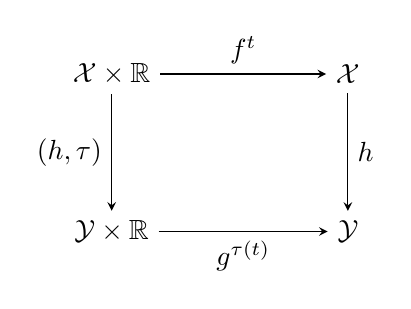
\begin{tikzpicture}[>=stealth, every node/.style={draw=none}]
  % Nodes
  \node (X1) at (0, 2) {$\mathcal{X} \times \mathbb{R}$};
  \node (X2) at (3, 2) {$\mathcal{X}$};
  \node (Y1) at (0, 0) {$\mathcal{Y} \times \mathbb{R}$};
  \node (Y2) at (3, 0) {$\mathcal{Y}$};

  % Arrows
  \draw[->] (X1) -- node[above] {$f^t$} (X2);
  \draw[->] (X1) -- node[left] {$(h,\tau)$} (Y1);
  \draw[->] (X2) -- node[right] {$h$} (Y2);
  \draw[->] (Y1) -- node[below] {$g^{\tau(t)}$} (Y2);
\end{tikzpicture}
\end{center}
Having this foundation allows us to more precisely describe the geometry of the dynamical system. First up, we shall see that the dynamical system has a very particular structure locally around stationary points. Stationary points serve a parallel purpose to those defined in introductory calculus. For us, we will understand them as follows:
\begin{mydefinition}{Stationary Points}
Let $F:\mathcal{X}\to \mR^d$ be a $C^1$ vector field with $\mathcal{X}\subset \mR^d$ open. We say that
\begin{itemize}
	\item $p\in \mathcal{X}$ is \emph{stationary} if $F(p)=0$,
	\item a stationary point $p\in \mathcal{X}$ is \emph{simple} if the Jacobian $DF(p)$ has full rank,
	\item a simple stationary point $p\in \mathcal{X}$ is \emph{hyperbolic} if all the eigenvalues of $DF(p)$ have non-zero real parts,
	\item a hyperbolic stationary point is an \emph{attractor} if all eigenvalues of $DF(p)$ have negative real parts,
	\item a hyperbolic stationary point is a \emph{repeller} if all eigenvalues of $DF(p)$ have positive real parts, and
	\item a hyperbolic stationary point is a \emph{saddle point} if it is neither an attractor nor a repeller.	
\end{itemize}
\end{mydefinition}
It is straightforward to see that if $p$ is a stationary point of a $C^1$ vector field, then $p$ is a fixed point of the time $t$-maps of the dynamical system arising from the autonomous differential equation \ref{diffeqvf}, i.e. $f^t(p)=p$. Moreover, it is not too hard to show that $Df_p(t)=\exp(tDF(p))$ with $f_p$ the trajectory of $p$. This allows us to translate the properties in terms of the vector field into properties in terms of the flow. With this terminology settled, we will now look at how these definitions correspond to geometric properties of flows around stationary points. One classical result is the Grobman-Hartman theorem:
\begin{thm}[Grobman-Hartman Theorem for Flows]
Let $p\in \mathcal{X}$ be a hyperbolic stationary point of a $C^1$ vector field $F:\mathcal{X}\to\mR^d$. Then there exist neighborhoods $\mathcal{V}$ of $p$ and $\mathcal{W}$ of $0\in \mR^d$, and a topological conjugacy $H:\mathcal{V}\to\mathcal{W}$ with $H(p)=0$ conjugating the flow of $F$ restricted to $\mathcal{V}$ to the flow of the linear vector field $A=DF(p)$ restricted to $\mathcal{W}$.
\end{thm}
This theorem shows that we can linearize the flow around stationary points, which in turn gives way for a much richer description of the geometry of the flow. We find that that we can aptly describe this structure with the theory of manifolds. The key reasoning behind this result, is that the we can extrapolate behaviour around the fixed points of a flow from the linearization given by the Grobman-Hartman Theorem. We record all this structure in the following result, which is also the main result of this theoretical section and links the theory of dynamical systems with the theoretical results on state space reconstruction, we will consider in the rest of chapter. It goes as follows:
\begin{thm}[Stable Manifold Theorem]\label{stable}
Let $F:\mathcal{X}\to \mR^d$ be a $C^k$ vector field, $k\geqslant 1$, at let $p\in \mathcal{X}$ be a hyperbolic stationary point, and let $A:\mR^d\to\mR^d$ be the linear map $x\mapsto DF(p)x$. Moreover, let $(f^t)_t$ be the flow of $F$. Then there exists invariant subspaces $E^s,E^u\subset\mR^d$, satisfying that 
\begin{enumerate}[label=(\roman*)]
	\item $E^s,E^u$ decompose $\mR^d$: $\mR^d=E^s\oplus E^u$,
	\item $E^s,E^u$ are invariant under $A$: $A(E^s)\subset E^s$ and $A(E^u)\subset E^u$,
	\item all eigenvalues of a matrix representing $A|_{E^s}$ have negative real parts, and all eigenvalues of a matrix representing $A|_{E^u}$ have positive real parts.
\end{enumerate}
Moreover there exist injective $C^k$ maps $\psi^s: E^s\to \mathcal{X}$ and $\psi^u:E^u\to\mathcal{X}$ satisfying that
\begin{enumerate}[label=(\roman*)]
\setcounter{enumi}{3}
	\item $\psi^s(0)=\psi^u(0)=p$,
	\item $D\psi^s(0)E^s=E^s$ and  $D\psi^u(0)E^u=E^u$,
 \item $\psi^s,\psi^u$ are of maximal rank: for all $u\in E^s$, $$\rank D\psi^s(u)=\dim E^s$$ and for all $v\in E^u$, $$\rank D\psi^u(v)=\dim E^u,$$
 \item and the images of $E^s/E^u$ under $\psi^s/\psi^u$ are attracting/repelling:
 \begin{align*}
  \psi^s(E^s)&=\{x\in \mathcal{X}:\lim_{t\to\infty}f^t(x)=p\},\\
 \psi^u(E^u)&=\{x\in \mathcal{X}:\lim_{t\to\infty}f^{-t}(x)=p\}
 \end{align*}
\end{enumerate}
\end{thm}
This theorem implies that if we have reason to believe that we are observing trajectories from a dynamical system that converge to some steady state or limit, then the theorem above realizes that trajectory on a suitable set, that has a lot of structure. We will quickly see that these sets are in fact manifolds, as we are about to define. As for the proofs of the Grobman-Hartman theorem and the stable manifold theorem, we refer once more to \cite{Dynamics}. Before that, there are several important remarks to make to this theorem:
\begin{itemize}
	\item If $p$ is an attractor, then we see that $E^s$ is all of $\mR^d$, and if $p$ is a repeller, then $E^u$ is all of $\mR^d$. In particular, if $p$ is an attractor, we observe by the mere fact that $\mathcal{X}\subset \mR$ that the attractor set $\psi^s(E^s)$ is a neighbourhood of $p$, so everything around $p$ will converge to this point. 
	\item If $\mathcal{X}$ is compact and convex, then it is a consequence of Brouwer's fixed point theorem that a time $t$-map $f:\mathcal{X}\to\mathcal{X}$ has a fixed point $p\in \mathcal{X}$, and if it is hyperbolic this activates the stable manifold theorem. This is in fact a stronger statement than that of the stable manifold theorem, since it implies the latter by the correspondence between fixed points of time $t$-maps of a vector field and stationary points of the vector field.
	\item It is a generic property that a linear map $\mR^d\to\mR^d$ is hyperbolic, meaning that the set of hyperbolic linear vector fields is an open and dense set of the space $\mathcal{L}(\mR^d,\mR^d)$ equipped with any topology induced by a norm: for instance one could go the matrix representation and use the matrix norm. This is the first example of a generic property in this thesis, but we shall see that this a typical concept in this setting.
\end{itemize}
We see that the stable manifold theorem can be more eloquently formulating in the language of manifolds. In practice, the manifolds we will consider can always be thought of as subspaces of $\mR^d$ for a suitable dimension $d\in \mN$, but it does help somewhat in the eloquence and not much intuition is lost. To that end, we do some heavy lifting now in generalizing the basic concepts from calculus to the world of differential topology and manifolds in order to better formulate the theorems in subsequent sections:
\begin{mydefinition}{Manifolds}
Let $M$ be a separable Hausdorff space and let $m\in \mN$.\\[5pt]
We call $(U,h)$ a \emph{chart} if $U\subset M$ is open and $h: U\to \mR^m$ is a homeomorphism onto its range with $U$ the \emph{chart domain} and $h$ the \emph{coordinate function}.\\[5pt]
If for each point $x\in M$, there exists a chart $(U,h)$ on $M$ such that $x\in U$, we call $M$ a \emph{manifold of dimension $m$}, and we call a collection of charts whose chart domains cover all of $M$ an \emph{atlas}.The collection of all charts on $M$ is itself an atlas that we call the \emph{structure} on $M$.\\[5pt]
On overlapping chart domains of charts $(U,h)$ and $(V,g)$, we consider the \emph{coordinate transformations}
$$hg^{-1}: g(U\cap V)\to \mR^m, \text{ and } gh^{-1}: h(U\cap V)\to \mR^m$$
We say the charts are \emph{$C^r$-related} if the coordinate transformations $hg^{-1}, gh^{-1}$ are $C^r$, and if all coordinate transformations of an atlas are $C^r$-related, we say the atlas is \emph{$C^r$-differentiable}. A \emph{differential structure} is the set of all charts $C^r$-related to the charts in some atlas. We shall say a manifold is $C^r$ if there exists a $C^r$-differentiable atlas of $M$.\\[5pt]
If $M$ is $C^r$ and $N$ is a $C^r$ manifold of dimension $n\geqslant m$, the function $f: M\to N$ is \emph{$C^r$-differentiable} if for each $p\in M$, there exists charts $(U,h)$ on M and $(V,g)$ on N, such that $p\in U$, $f(p)\in V$ and 
$$gfh^{-1}: h(U\cap f^{-1}(V))\to \mR^n$$
is $C^r$. (Remark: this property thus holds for any choice of charts in the atlas covering $p$ and $f(p)$ respectively). The \emph{Jacobian} at $p$ is then defined as 
$$Dgfh^{-1}(h(p))$$
This depends on the choice of charts but the rank does not.\\[5pt]
If the Jacobian is of maximal rank (rank $m$), we say $f$ is \emph{immersive at p}, and if $f$ is immersive everywhere, then we say $f$ is an \emph{immersion}. An immersion that is homeomorphic upon its image is an \emph{embedding}.\\[5pt]
Conversely, if $m\geqslant n$, and the Jacobian is of maximal rank (rank $n$), then $f$ is \emph{submersive at $p$}, and if submersive everywhere it is a \emph{submersion}. If $f: M\to N$ is an embedding, we say that $f(M)$ is a \emph{submanifold} of $N$.\\[5pt]
A \emph{diffeomorphism} is a map $f:M\to N$ for which there exists a differentiable inverse, and in this case we shall call $M$ and $N$ \emph{diffeomorphic}. If $f$ is an embedding, it is possible to prove that $f:M\to f(M)$ is a diffeomorphism.\\[5pt]
Finally, we will define some topologies. We let $C^r(M,N)$ denote the space of all $C^r$ differentiable maps from $M$ to $N$. We then let the topology of $C^r(M,N)$ be generated by the subbase consisting of sets defined as follows: for any choice of function $f\in C^r(M,N)$, charts $(U,h)$ on $M$ and $(V,g)$ on $N$, a compact set $K\subset U$ such that $f(K)\subset V$ and $\varepsilon>0$, we define $\mathcal{N}(f,(U,h),(V,g),K,\varepsilon)$ to be the set of all functions $\hat{f}\in C^r(M,N)$ for which $\hat{f}(K)\subset V$ and
$$\norm{D^kg\hat{f}h^{-1}(x)-D^kgfh^{-1}(x)}<\varepsilon$$
for all $x\in h(K)$, $k=0,\ldots,r$, where $\norm{\cdot}$ is the usual Euclidean norm. If $M$ and $N$ are diffeomorphic, we let $\text{Diff}^r(M,N)$ be the subspace of $C^r(M,N)$ consisting of $C^r$-differentiable diffeomorphisms equipped with the subspace topology. Usually, we will use the shorter $\text{Diff}^r(M)$ for $\text{Diff}^r(M,M)$.
\end{mydefinition}
We recognize immediately that the maps $\psi^s$ and $\psi^u$ of the stable manifold theorem (\ref{stable}) are injective $C^k$ immersions, and that the attractor and repeller sets $W^s(p)\coloneqq \psi^s(E^s)$ and $W^u(p)\coloneqq \psi^u(E^u)$ are indeed manifolds, that we usually call respectively the \emph{stable manifold} and the \emph{unstable manifold}. We recognize a certain likeness to the limiting distributions leading to undirected edges when working with chain graphs from the idea of attractor sets in the dynamical systems world. We end this section by extending the theory of dynamical systems to this manifold setting:
\begin{mydefinition}{Differential Equations on Manifolds}
A \emph{vector field} on a manifold $M$ is a map $F:M\to TM$, and a \emph{differential equation} is given by
\end{mydefinition}
We solve differential equations on manifolds by localization on charts, using the results from theorem \ref{ThmDiffEq} to generate solutions. Of course some technicalities arise in this context, but it is mainly a matter of looking at the behavior on overlapping charts and using the properties of the coordinate transformations. In all essence, we can give the following analogy of theorem \ref{ThmDiffEq}:
\begin{thm}[Solutions to Differential Equations on Manifolds]\label{ThmManifDiffEq}
Fix $d\in \mN$. Let $F:\mathcal{U}\to\mR^d$ be a continuous function with $U$ an open subset of $\mR^{1+d}$. We consider the following differential equation for differentiable $x:\mR\to\mR^{d}$:
\begin{equation}\label{diffeq}
x'(t)=F\left(t,x(t)\right)
\end{equation}
We then have the following results:
\textbf{Peano's theorem:} For every $(t_0,x_0)$ there exists a solution on some open interval $I$ to the differential equation \ref{diffeq} going through $x_0$ at $t_0$, meaning that:\\
	For every $(t_0,x_0)\in \mathcal{U}$, there exist an open interval $I$ and a differentiable function $\gamma: I\to \mR^d$, such that $t_0\in I$, $\gamma(t_0)=x_0$ and for all $t\in I$
		$$\gamma'(t)=F\left(t,\gamma(t)\right)$$

\end{thm}

\section{Takens' Theorem}
In the following, we will switch gears from the more welcoming realm of considering functions in $\mR^n$ and $\mR$ and move to the realm of differential topology, which is inhabited by manifolds, vector fields and tangent bundles and worse. This is done, not for needless abstraction, but because the theory we shall be exploiting holds in this generality - and in fact as long we consider compact manifolds, we might as well think of them in Euclidean spaces nonetheless. So in practice, we will always be able to envision our models living in our usual space $\mR^n$, but it is not in any way useful to restrict ourselves at this point.\\
We will consider different setups, but the base model is systems modelled as vector fields on invariant compact manifolds (separable, Hausdorff, locally Euclidean spaces), which can be generalized to cover vector fields with an attractor set, that need not in fact be a manifold, see \cite{Sauer1991}. As the theorem itself, this is formulated in the realm of differential topology and so the objects involved in the theorem and subsequqnt theory spring from there. Below we will briefly introduce and recite the definitions of the objects of relevance, if nothing else to clarify the terminology used in this thesis. In practice, most of our examples will come from partial differential equations (PDEs) and stochastic differential equations (SDEs); we will consider the link between these realms in more detail later. We will for now interpret the manifold as the 'path' of the system, that is the values that the system takes throughout time. With terminology borrowed from physics, one could call this the \textit{phase space}. The fundamental result we shall use, now known as Takens' theorem, was proved in 1981 by Floris Takens, \cite{Takens}, and states that one can reconstruct the manifold using only a univariate observation function; that is observing only one variable over time allows us to reconstruct the entire path of the dynamic system of all variables. The original theorem as stated by Takens is as follows:
\begin{thm}[Takens, Version 1]
Let M be a compact manifold of dimension $m$. For pairs $(\varphi,y)\in \text{Diff}^2(M)\times C^2(M,\mathbb{R})$, it is a generic property that the map $\Phi_{(\varphi,y)}:M\to \mathbb{R}^{2m+1}$, defined by
$$\Phi_{(\varphi,y)}(x)=(y(x),y(\varphi(x)),...,y(\varphi^{2m}(x))),$$
is an embedding. \cite{Takens}
\end{thm}
There are several things to unpack here. First of all, it is worth noting the differentiability constraints on our maps; both $\varphi: M\to M$ and $y:M\to\mR$ are required to be twice continuously differentiable. In the work of \cite{Sauer1991}, their setup enables this requirement to be relaxed to them only being once continuously differentiable. Our dynamical system is indeed a vector field on an invariant compact manifold being the first regularity condition, this is then the second regularity condition, that we will for the most part silently have to assume is fulfilled. Next, we will call $y$ our \textit{observation function}, and we can think of this as a series of observations made from the system. For now, $\varphi$ remains a bit more mysterious, but we shall quickly make this map must more explicit. We shall call $\Phi$ for the \textit{delay embedding}, the reasoning behind which will be revealed shortly. However, the most important caveat is perhaps that it is 'only' a generic property that the theorem yields an embedding. We will provide more rigorous definitions later, but for now we will understand embedding simply as a reconstruction of the manifold. By generic property is meant to be understood that for 'most' observation functions $y$ and most choices $\varphi$, the delay embedding is indeed an embedding. The precise meaning in an algebraic sense is that there exists an open and dense subset of the function space $C^2(M,\mR)$, respectively $\text{Diff}^2$, for which the statement is true. From this stems our second regularity assumption. For $\varphi$, we will be able to do some reasoning in practical cases, but for $y$ this will often be just another silent assumption. We shall be calling a map $y\in C^2(M,\mR)$, respectively $\varphi\in \text{Diff}^2(M)$, \textit{generic} if there exists $\varphi\in \text{Diff}^2(M)$, respectively $y\in C^2(M,\mR)$, such that the resulting delay embedding is indeed an embedding.\\\\
We will now work towards a more explicit version of the theorem. First of all, the reasoning behind the naming of the delay embedding, comes from the following: we shall associate any given time point $t\in \mR_{\geqslant 0}$ with a position $x(t)\in M$ on the manifold. For a given delay length $\tau\in \mR_{>0}$, we may then define $\varphi_\tau: M\to M$ by $x(t)\mapsto x(t-\tau)$. Substituting this into Takens' theorem reduces the delay embedding to
$$\Phi(x(t))=(y(x(t)),y(x(t-\tau)),\ldots,y(x(t-2m\tau)))$$
Takens' theorem thus states that the values of a single time series considered at different delays will reconstruct the manifold 'generically'. Now we will need to ensure that this choice of $\varphi$ is both twice continuously differentiable and is not of such a nature that it falls out of the set of generic functions. The differentiability constraint falls under the umbrella of regularity assumptions, while we can guarantee that $\varphi_\tau$ will be generic for some choices of $\tau$ by the power of a restatement of Takens' theorem. It was in fact proved by Takens in \cite{Takens}, but not stated. We will follow the restatement of the theorem as well as the subsequent presentation of theory and definitions presented in \cite{Huke} for the rest of this section.
\begin{thm}[Takens, version 2]
Let M be a compact manifold of dimension $m$. Let $\varphi\in\text{Diff}^2(M)$ satisfy
\begin{enumerate}[label=\arabic*)]
	\item the periodic points of $\varphi$ with periods less than or equal to $2m$ are finite in number,
	\item if $x$ is any such periodic point with period $k\leqslant 2m$, then the eigenvalues of $\varphi^k$ at $x$ are all distinct.
\end{enumerate}
 Then it is a generic property for $y\in C^2(M,\mR)$ that the map $\Phi_{(\varphi,y)}:M\to \mathbb{R}^{2m+1}$, defined by
$$\Phi_{(\varphi,y)}(x)=(y(x),y(\varphi(x)),...,y(\varphi^{2m}(x))),$$
is an embedding. \cite{Huke}
\end{thm}
By periodic with period less than or equal to $2m$, we mean that $\varphi^{k}(x)=x$ for some $k\leqslant 2m$. If $\tau$ is chosen such that there are no periodic points of $\varphi_\tau$, or if we assume some structure on the periodic points, then we need only worry about whether $y$ is generic. In fact, if $\varphi_\tau$ is not generic for some choice of $\tau$, it will usually be after some small perturbation in $\tau$ (\textit{is it true, reference?}). Therefore in practice multiple lags can be tested, and we should thus be able to fairly easily sidestep this problem. Before moving on to definitions and technicalities, we will at this point however notice that we have a theorem that gives an explicit construction that will fairly generally allow us to completely recover the dynamics of a system from only a single variable observed over time. In contrast to the choice of $\tau$, we will however usually have in practice that the observation functions are fixed. So even if the same technique of small perturbations of a non-generic observation function produces a generic observation, we do not have access to it. Therefore we will usually have to assume a given observation function is generic, if there is no reason to believe otherwise. However, in some cases we can actually endow genericity with causal interpretation - we return to this in the next section. For now, we expand upon Takens' theorem.  We start of with the basic definitions needed following very closely the terminology and presentation from \cite{Huke2}. 


Before moving on, we will outline the main stages in Takens' theorem just to get an understanding of the proof techniques. In the following, we will use the subspace topology on $C^2(M,\mR)$ inherited from $C^1(M,\mR)$ and likewise on $\text{Diff}^2(M)$. In all topological statements below, this is what is meant. We proceed by proving the 2nd version of Takens' theorem as follows:
\begin{enumerate}[label=\roman*)]
	\item The first stage hangs on using the following standard fact in differential topology:
	\begin{thm}
	Let $M$ be a compact manifold, and let $N$ be any manifold. The set of $C^r$ embeddings of $M$ in $N$ is open in $C^r(M,N)$. \cite{hirsch}
	\end{thm}
	Proving that the map $\mathcal{F}^2: C^2(M,\mR)\to C^2(M,\mR^{2m+1})$, defined by $$y\mapsto (y,y\circ\varphi,\ldots, y\circ \varphi^{2m}),$$ 
	is continuous then immediately proves that the set of generic observation functions is open in $C^2(M,\mR)$. This is done in the following familiar set of steps: one proves $F: C^2(M,\mR)\to C^2(M,\mR)$ defined by $y\mapsto y\circ\varphi$, for $\varphi\in \text{Diff}^2(M)$, is in fact continuous.  This is simply a matter of unravelling the definition of the topology above, and requires only a slight bit of trickery. We skip the details of these derivations. By induction, it follows that $F_n:  C^2(M,\mR)\to C^2(M,\mR)$ defined by $y\mapsto y\circ\varphi^n$ is in fact continuous.  The final detail is to use that the product topology of $C^r(M,\mR)^{2m+1}$ coincides with that of $C^r(M,\mR^{2m+1})$. Worth remarking here is that we have made no assumptions on $\varphi$ yet, any embedding will do. Likewise, we have not used $m$ to do anything yet. 
\end{enumerate}
The following technical fact will prove fairly useful - and it is just a matter of exploiting the compactness of $M$ and using the definition of the topology. If $y\in C^2(M,\mR)$, and $\psi_i\in C^2(M,\mR)$, $i=1,\ldots,N$ for some $N\in \mN$. Then for every neighbourhood $\mathcal{N}$ of $y$, there exists $\delta$ such that
$$y+\sum_{i=1}^N a_i\psi_i\in \mathcal{N}$$
for all $a=(a_1,\ldots,a_n)$ with $\norm{a}< \delta$. 
\begin{enumerate}[label=\roman*)]
	\setcounter{enumi}{1}
	\item The following stages all revolve around exploiting this fact. To prove that the set of generic functions are dense, we consider an arbitrary $y\in C^2(M,\mR)$ and a neighbourhood $\mathcal{N}_y$ of $y$. Now we want to identify a generic observation function in $\mathcal{N}_y$. First, we return to the conditions of the 2nd version of Takens' theorem. Let us denote the points with period less than or equal to $2m$ by $P_{2m}$. Since $|P_{2m}|<\infty$, we know by the Hausdorff property of $M$, that we can find pairwise disjoint neighbourhoods of the elements in $P_{2m}$, and so by a fairly standard argument we can separate these points by observation functions, and we use the fact above. Now we have $y'\in\mathcal{N}_y$ that is injective on $P_{2m}$. Similarly, by doing some explicit calculations on the Jacobian, we can identify a function $y''$ not only injective but also immersive on $P_{2m}$. To be continued...
	\item The proof of the 1st version of Takens' theorem from the 2nd version consists of utilising the Kupka-Smale theorem, namely that it is a generic property that for $\varphi\in \text{Diff}^2(M)$ and some integer $n\in \mN$, the number of periodic points, with period $n$ or less, is finite. There is a little in work in showing that this extends to cover the second condition of the 2nd version, and one also needs to use an argument similar to that in stage i) to prove the openness claim in $\text{Diff}^2(M)\times C^2(M,\mR)$ instead of just in $C^2(M,\mR)$. But the main component is the Kupka-Smale theorem.
\end{enumerate}  
Takens' theorem will allow us to do causal inference in the modelling framework introduced in this chapter. Below we give the theoretical details of this procedure.
\section{Causal Inference with Takens' Theorem}
In this section, we will show that we can only hope to recover the component graph from data using Takens' theorem. We shall later discuss attempts to reason further about the causal structure, but the results below will show that without further assumptions, we cannot distinguish direct and indirect causal links.\\\\
The aim of this section is to show that under suitable regularity assumptions, we can create a correspondence between strongly connected components and sub-manifolds, and that this correspondence is precisely fine-grained enough to allow us to determine whether any two variables belong to the same strongly connected component and further the direction of the causal link if they do not. To do this, we have to formalize this correspondence. First of all, as discussed the component graph $CG_\varphi$ is a directed acyclic graph, and so we can think of the graph structure as a partial order, where $x,y\in CG_\varphi$ satisfy $y\geqslant x$ if $y\to x$. Considering then the upper sets, we inherit an ordering of these, since they are exactly defined with respect to the partial order, and since we are dealing with sets, we can unproblematically consider the union and intersection of upper sets. This structure is that of a lattice:

\begin{defn}[Driver]
Given a dynamical system $\varphi$, and two variables $x$ and $y$ of $\varphi$, the variable $x$ \emph{directly drives} $y$ if the dynamics of $y$ directly depend on $x$, that is $y_{t+1}=g(x,\cdot)$ for discrete systems and $\dot{y}=g(x,\cdot)$ for continuous.
\end{defn}
\begin{defn}[Component graph]
A subset of vertices $W\subset V$ of the interaction graph is called a \emph{strongly connected component}, if for any $u,v\in W$ there exists a directed path from $u$ to $v$ and a directed path from $v$ to $u$. We define the \emph{component graph} as the graph obtained from the interaction graph by taking the set of strongly connected components $\mathcal{S}$ as the set of vertices, and letting there be a directed edge from $p\in \mathcal{S}$ to $q\in \mathcal{S}$ if there exists a $u\in p,v\in q$ such that there exists a directed path from $u$ to $v$.
\end{defn}
Note that being strongly connected defines an equivalence relation. The component graph will turn out to be very relevant in the following analysis.
It will turn out that each upper set corresponds to a self-contained dynamical system. The final component in our later analysis is the so-called \textit{transitive closure}:
\begin{defn}[Transitive closure]
Given a DAG $\mathcal{G}=(\mathcal{V},\mathcal{E})$, the \emph{transitive  closure of $\mathcal{G}$} is the graph obtained from $\mathcal{G}$ by taking the vertices $\mathcal{V}$ and include the edge between $u\in \mathcal{V}$ and $v\in \mathcal{V}$ if and only if there is a directed path from $u$ to $v$.
\end{defn}
The transitive closure of a causal graph encodes only the causal direction between variables but cannot distinguish between direct and indirect causal links. In other words, from the transitive closure you can infer all descendants of a given variable, but not the causal graph itself. It will turn out that this is exactly what we will be able to recover with the modelling framework based on Takens' theorem.\\[10pt]
\begin{defn}[Lattice]
A \emph{lattice} $L$ is a partially ordered set if for every two elements $a,b\in L$, there exists a least common upper bound, called a \emph{join}, denoted $a \vee b$ and a greatest common lower bound, called a \emph{meet}, denoted $a\wedge b$. Further, we require that if $a_1\leqslant a_2$ and $b_1\leqslant b_2$, then
$$a_1\wedge b_1\leqslant a_2\wedge b_2$$
and
$$a_1\vee b_1\leqslant a_2\vee b_2$$
We shall call $L$ \emph{distributive}, if
$$a\wedge(b\vee c)=(a\wedge b)\vee (b\wedge c)$$
\end{defn}
We see that we can think of the set of upper sets as a lattice when equipping it with unions and intersections. This lattice is going to be the index set for our subdivisions of manifolds, and so this will give us a natural way to think of the causal structure. We introduce the notion of a filtration:
\begin{defn}[Filtration]
Let $I$ be a partially ordered set, and let $(X_i)_{i\in I}$ be a collection of topological spaces and let further $(\iota_{ij})_{j\leqslant i}$ be a family of continuous maps $\iota_{ij}: X_i\to X_j$ satisfying the consistency constraint
$$\iota_{ik}=\iota_{ij}\circ \iota_{jk}$$
Then $(X_i,\iota_{ij})_I$ is an \emph{inverse system}, and we will also refer to it as a \emph{filtration}. An inverse system indexed by $I'$ obtained from $I$ by reversing all relations will be called a \emph{descending filtration} on $(X_i)_I$.
\end{defn}
This allows us to consider the causal structure as an object, and we can now use this object to create the correspondence discussed above. We will now define a descending filtration on the phase space. For this, we shall utilize that we can think of any compact finite dimensional manifold as a subspace of $\mR^n$ for suitable $n$, in fact this very fact is implied by Takens' theorem, and we shall think of the observed values as the coordinates of $\mR^n$. This reduces the generality of the approach somewhat, but it lends itself to interpretability and the modelling framework introduced in the beginning of this chapter. This leads us to the definition of a descending filtration of the phase space:
\begin{defn}[Upper set filtration]
Let $UL_\varphi$ be the lattice imposed by considering the upper sets of the component graph of a dynamical system $\varphi$. For $U\in UL_\varphi$, we define $|U|$ as the set of all variables contained the upper set $U$ and we will call it \textit{variable set} of $U$. Further, we let $\mR_U$ be the space spanned by $|U|$ of dimension $\#|U|$ and we call this the \textit{phase space} of $U$. We see now that for $U,V\in UL_\varphi$, we have $U\leqslant V$ if and only if $|U|\subset |V|$, which in turn is equivalent with $\mR_U\subset \mR_V$. We thus get a natural projection $\pi_{VU}:\mR_V\to\mR_U$. We further define $\pi_U$ as the natural projection $\mR^n\to \mR_U$. We see that this defines a descending filtration, and we call $(\mR_U,\pi_{UV})_{UL_\varphi}$ the \emph{upper set filtration of the phase space}.
\end{defn} 
\begin{prop}
Given a causal (\textit{definition!!}) dynamical system $\varphi$, and upper sets $U,V\in UL_\varphi$ with $U\leqslant V$, the family of maps $\{\varphi^t_W\}_{W\in UL_\varphi}$, where $\varphi_U^t$ is defined on $\mR_U$ and given by the equation
$$\varphi^t_U\circ\pi_U(x)=\pi_U\circ \varphi^t(x)$$
for all $x\in \mR$, is well-defined, and the the collection $(\mR_U,\pi_{UV})_{UL_\varphi}$ of dynamical systems is consistent, meaning that they satisfy
$$\pi_{VU}\circ \varphi_V^t(x)=\varphi_U^t(x)\circ\pi_{VU}(x)$$
for all $x\in \mR_V$.
\end{prop}
\begin{proof}
Suppose $\pi_U(x)=\pi_U(y)$ for $x,y\in \mR^n$. Hence $x,y$ differ in the variables $|\mathcal{V}_\varphi|\setminus |U|$, and since $U$ is an upper set, it follows that $\pi_U(\phi^t(x))=\pi_U(\phi^t(y))$, since the values of $\varphi^t$ on the variable set $|U|$ does not depend on the variables  among $|\mathcal{V}_\varphi|\setminus |U|$.\\
Observe that since each $x\in \mR_V$ can be written as $\pi_V(x')$ for some $x'\in \mR$, and since we can rewrite
\begin{align*}
\pi_U\circ\varphi^t(x')
&=\varphi_U^t(x)\circ\pi_U(x')=
\varphi_U^t\circ\pi_{VU}\circ\pi_V(x')=\varphi_U^t\circ\pi_VU(x),\quad\quad \text{and}\\
\pi_U\circ\varphi^t(x')&=\pi_{VU}\circ \pi_V\circ\varphi^t(x')=\pi_{VU}\circ \varphi_V^t\circ \pi_V(x')=\pi_VU\circ\varphi_V^t(x)
\end{align*}
by consistency of the upper set filtration, we get consistency of the collection as desired.
\end{proof}
This allows us to introduce a filtration of the manifolds on which our models live:
\begin{defn}
Let $\varphi$ be a dynamical system restricted to a compact invariant manifold. Then we will call the descending filtration $\{M_U\}_{U\in UL_\varphi}$, with $M_U$ defined by $M_U\coloneqq \pi_U(M)$, equipped with the family of maps $\pi_{VU}$, for the \emph{invariant set filtration} $\mathbb{M}$.
\end{defn}
We notice immediately that for any $U\in UL_\varphi$, then $M_U$ is a compact invariant set for the dynamical system $\varphi^t_U$. We can now decompose our dynamical systems into smaller dynamical systems based on the causal structure, and we now give a similar decomposition of the observation functions:
\begin{defn}[Filtration of observation functions]
For $U\in UL_\varphi$, let $Y_U\coloneqq C^2(M_U,\mR)$ denote the set of observation functions on $M_U$, and define $\iota_{UV}:Y_U\to Y_V$ by $\iota_UV(\varphi)=\varphi\circ \pi_{VU}:M_V\to \mR$. We call this the \emph{filtration of observation functions} and denote it $\mathbb{Y}$.
\end{defn}
To complete the journey towards the main theorem of this chapter, we need some technical results to allow us to use Takens' theorem repeatedly for each manifold in the filtration. This is not of particular interest for the
\begin{prop}
The set of generic functions is open and dense bla bla
\end{prop}
We are approaching the full-fleshed formulation of our theorem now. We can now state the assumptions in full detail and the statement that allows us to identify causal statements
\begin{thm}[Identifiability in dynamic systems]
We assume the following of our dynamic system
\begin{enumerate}[label=(I\arabic*)]
	\item The elements $M_W$ of the invariant set filtration $\mathbb{M}$ are compact, invariant \emph{smooth} manifolds. 
	\item Given comparable $U,V$ in the lattice $UL_\varphi$ with $U<V$, the corresponding projection $\pi_{VU}:M_V\to M_U$ is non-injective.
	\item Given non-comparable $U,V$ in the lattice $UL_\varphi$, there exist no continuous surjections $f:M_U\to M_V$ or $g:M_V\to M_U$.
	\item We assume that $\varphi^T$ be generic for fixed $T$, and that $s$
\end{enumerate}
Let now $U,V$ be upper sets, let $\varphi_1,\varphi_2$ be corresponding observation functions and let $M_i=\Phi_{\varphi^T,y_i,k_i}(M)$ be the reconstructions, where $k_1\geqslant 2n_U$ and $k_2\geqslant 2n_V$. It then holds that:
\begin{enumerate}[label=\roman*.]
	\item $U=V$ if and only if there exists a homeomorphism
	$$\Psi_{1,2}:M_1\to M_2$$
	\item $U<V$ if and only if there exists a continuous surjective, noninjective map
	$$\Pi_{1,2}:M_2\to M_1$$ 
\end{enumerate}
\end{thm}
We have now proven that under conditions (I1)-(I4), it is actually possible to determine the causal directions in a dynamical system. The first condition is a regularity assumption that things are sufficiently well-behaved. We will give an alternative statement, where this condition is replaced, but in spirit this type of assumption is needed for any reconstruction to take place. It is the author's view that this is a reasonable assumption in most settings: although it might never actually be true that an observed system is restricted to a compact smooth manifold, we can think as we do in any kind of modelling as the imagined dynamic being a simplified representation of the system, and as far as the observed system behaves somewhat controlled locally, such a representation will probably be useful in capturing information about the system.\\\\ The second and third conditions are somewhat less reasonable in appearance; we are assuming the non-existence of mappings that if they existed would undermine the theoretical foundation of the theorem. This is undesirable. As is done in \cite{mathFound}, this is referred to the \textit{manifold being fully resolved}. An implied interpretation hereof is that it is simply matter of observing sufficient amounts of a data to separate different parts of the system - more on this later. This assumption is quite a standard one, and it is something that will appear in practical considerations nonetheless. A further comment on this, is that it corresponds somewhat to the faithfulness assumption often made when working with structural causal models.\\\\ The final assumption is entirely impossible to test as well, but we will interpret genericity in the same way as \textit{almost everywhere}, and assume that it is unlikely that we would ever get non-generic functions by accident. The almost everywhere interpretation is often a probabilistic one whereas this one is not, but as so often the difference is philosophical.\\\\
We have to in
\begin{cor}
Let $\varphi$ be a causal dynamical system, and let $UL_\varphi$ be the corresponding lattice. Assume that assumptions I1)-I4) are fulfilled for all elements in $UL_\varphi$. Then the following algorithm recovers the transitive closure of the component graph $CG_\varphi$:
\begin{enumerate}[label=\roman*.]
	\item Let the set of variables be the set of vertices in a graph we will call \emph{RG}.
	\item For every variable $x$, build the reconstructed manifold $M_x\coloneqq \Phi	_{(\varphi^T,x,k)(M)}$.
	\item For every pair $x$ and $y$, draw an edge $x\to y$ if there exists a continuous surjection $f:M_x\to M_y$ and draw an edge $y\to x$ if $g:M_y\to M_x$.
\end{enumerate}
\end{cor}
We remark the inherent simplicity of this approach as compared with Granger causality: in Granger causality, we have to account for all relevant information in order to allow for causal reasoning; here we need only consider the prints of the time series themselves. Of course, some potential problems may hide in our rather abstract set of assumptions I1)-I4). For instance, we cannot rule out a causal mirage due to synchronization: imagine a common causal confounder between two systems resulting in two heavily synchronized, but essentially 'independent' dynamic systems. This would result in erroneous causal interpretations, and so the problem of hidden confounders presents itself in this world as well. However, we would expect these mirages to occur only in the presence of heavy synchronization, so this potential undermining of causal inference may be less severe than in similar problems.\\\\ 
We used the term independent before, which of course is not to be interpreted in the probabilistic sense, as this is entirely meaningless in our setup; all our objects are deterministic, and they are all trivially independent in a probabilistic model. It is not quite true in a literal way either, since we assume that they are linked by a common cause; so all  that is meant that any further dynamic not imposed by the cause must be inherent to the subsystem and thus 'independent' of other subsystems.

\chapter{Convergent Cross Mapping}
Meanwhile we can exploit this idea of information being encoded in effect variables to great effect: this allows us to reformulate causality from the point of view of deterministic systems. The principle itself is fairly simple, but we do require some technical assumptions to make the theory work, which are not in any way empirically motivated nor entirely interpretable, but fare under what we usually consider regularity assumptions - a sweep-it-under-the-rug-interpretation would be that we just assume the data to be reasonably well-behaved. The basic idea is that if $C$ is the cause of $E$, then $E$ must contain information of $C$, since the dynamics of $C$ must be reflected in $E$ in light of a functional relationship, whereas the reverse cannot be true. Thus when reconstructing the entire dynamic system from the observed values of $E$ in accordance with the theorem, we would expect to recover the dynamics of $C$. We should however expect the reverse statement to be false, since the self-contained dynamics of $E$ would not be reflected in $C$, and so the dynamic system reconstructed from the observed values of $C$ would not recover the dynamics of $E$. Notice that this in fact implies the opposite of Granger causality: we should be able to predict the cause $C$ using the effect $E$ but not conversely. This is quite a radical difference. To obtain further understanding, we will have to delve into the theoretical details. 
\url{https://besjournals.onlinelibrary.wiley.com/doi/10.1111/2041-210X.13150}

\section{Implementation}
Takens' theorem implies that you can reconstruct the manifold by the map
$t\mapsto (y(t),y(t-\tau),...,y(t-L\tau))$
Using practical  
\subsection*{Reference Model}
We will use the following model built on a multivariate Ornstein-Uhlenbeck process as a reference. More specifically, we will consider the following setup. Let the $d$-dimensional stochastic process $X_t$, $t\geqslant 0$, be given by the following stochastic differential equation
$$dX_t=M X_t\ dt+\rho I_d\ dW_t$$
with $W_t$ a $d$-dimensional  Brownian motion, $M$ a $d\times d$ drift matrix, and $\rho\in \mathbb{R}$ a scalar. We will then consider observations at time points $0\leqslant t_1<t_2<\cdots <t_n$, $n\in \mathbb{N}$, with some observation noise
$$Y_{t_i}=X_{t_i}+\xi_i,\quad i=1,...,n$$
where $\xi_i$ is iid with $\mathbb{E} \xi_i=0$ and $V(\xi_i)=\sigma^2$ for some variance parameter $\sigma^2\in \mathbb{R}_{\geqslant 0}$. Interesting variations of this model, is $\sigma^2=0$, implying no observation noise, and $\rho=0$, which removes stochasticity of the process.
\section{Direct Extensions}


\section{Machine Learning Extensions}
\url{https://arxiv.org/pdf/nlin/0405016.pdf}\\[5pt]
\url{file:///C:/Users/rasmu/Downloads/s41598-021-87316-6.pdf}\\[5pt]
\url{https://static-content.springer.com/esm/art%3A10.1038%2Fs41598-021-87316-6/MediaObjects/41598_2021_87316_MOESM1_ESM.pdf}

\section{Dynamic Systems under Noise}
Consider the following generalization of the Ornstein-Uhlenbeck process:
$$du(t)=-Au(t)\ dt+F(u(t))\ dt+B u(t)\ dW_t,\quad t\geqslant 0$$
with the following assumption on $F:H\to H$
\cite{StableManifoldStoc} 

\section{Simulation Study}
\url{https://pure.au.dk/portal/files/136561486/Causal_inference_from_noisy_time_series_data_AM17.pdf}




\bibliographystyle{apalike2}
\bibliography{kilder}
\end{document}
